\documentclass[12pt,a4paper]{scrartcl}

\usepackage{graphicx} % includegraphic
\usepackage[left=1pt,right=1pt,top=1pt,bottom=1pt]{geometry} % define pagelayout

\usepackage{bookmark}
\usepackage{pdfpages}

\author{Ngoc Minh Dao}
\title{Zeugnisse}

\begin{document}
% Overide the margin from MyStyle settings
\bookmark[page=\thepage, level=-2]{Anlagenverzeichnis}
% Zeugnisse {{{
\bookmark[page=\thepage, level=-1]{Zeugnisse}

\bookmark[page=\thepage, level=0]{Arbeitszeugnis}
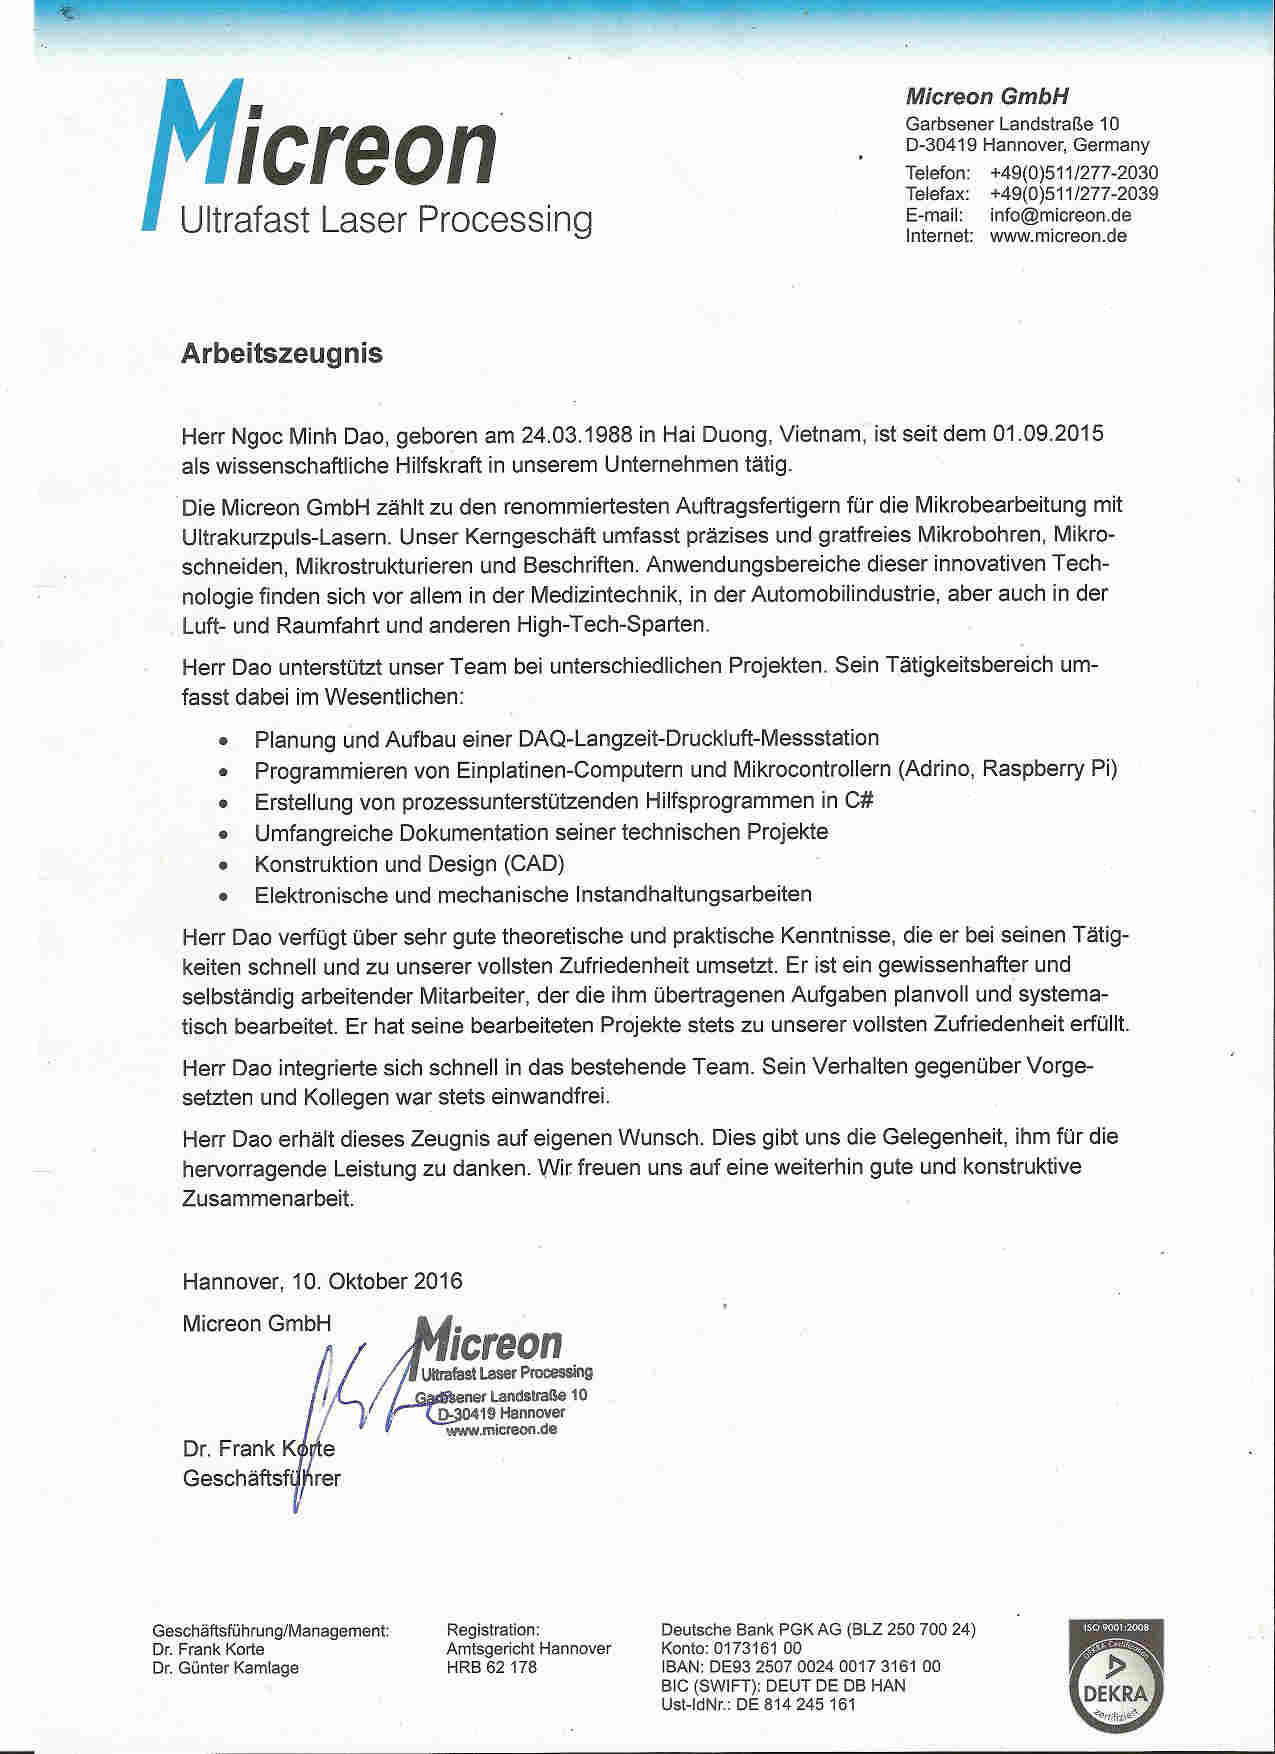
\includegraphics[width=\linewidth, height=\textheight, keepaspectratio]
{./zeugnisse/micreon_arbeitszeugniss_lq.jpg}

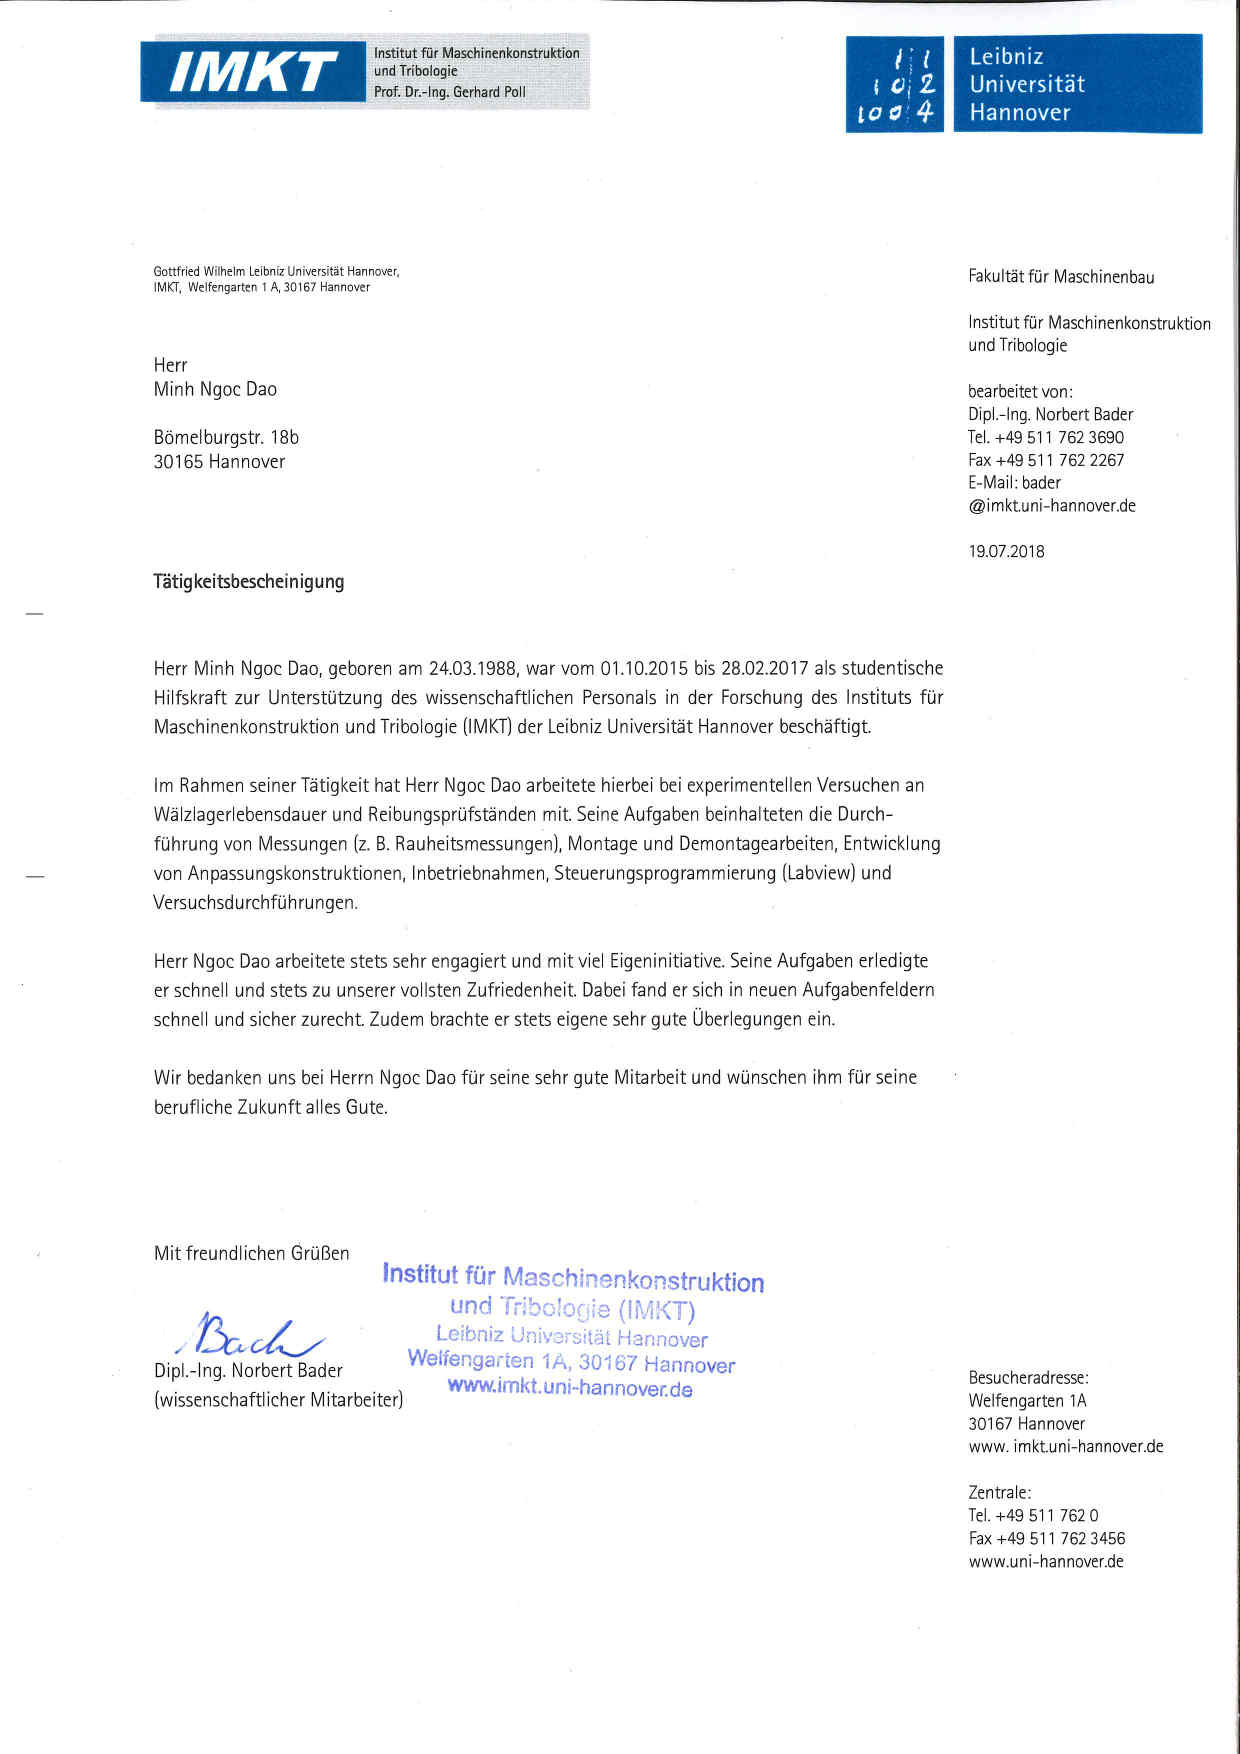
\includegraphics[width=\linewidth, height=\textheight, keepaspectratio]
{./zeugnisse/imkt_arbeitszeugnis_lq.jpg}

\newpage
\bookmark[page=\thepage, level=0]{Praktikumzeugnis}
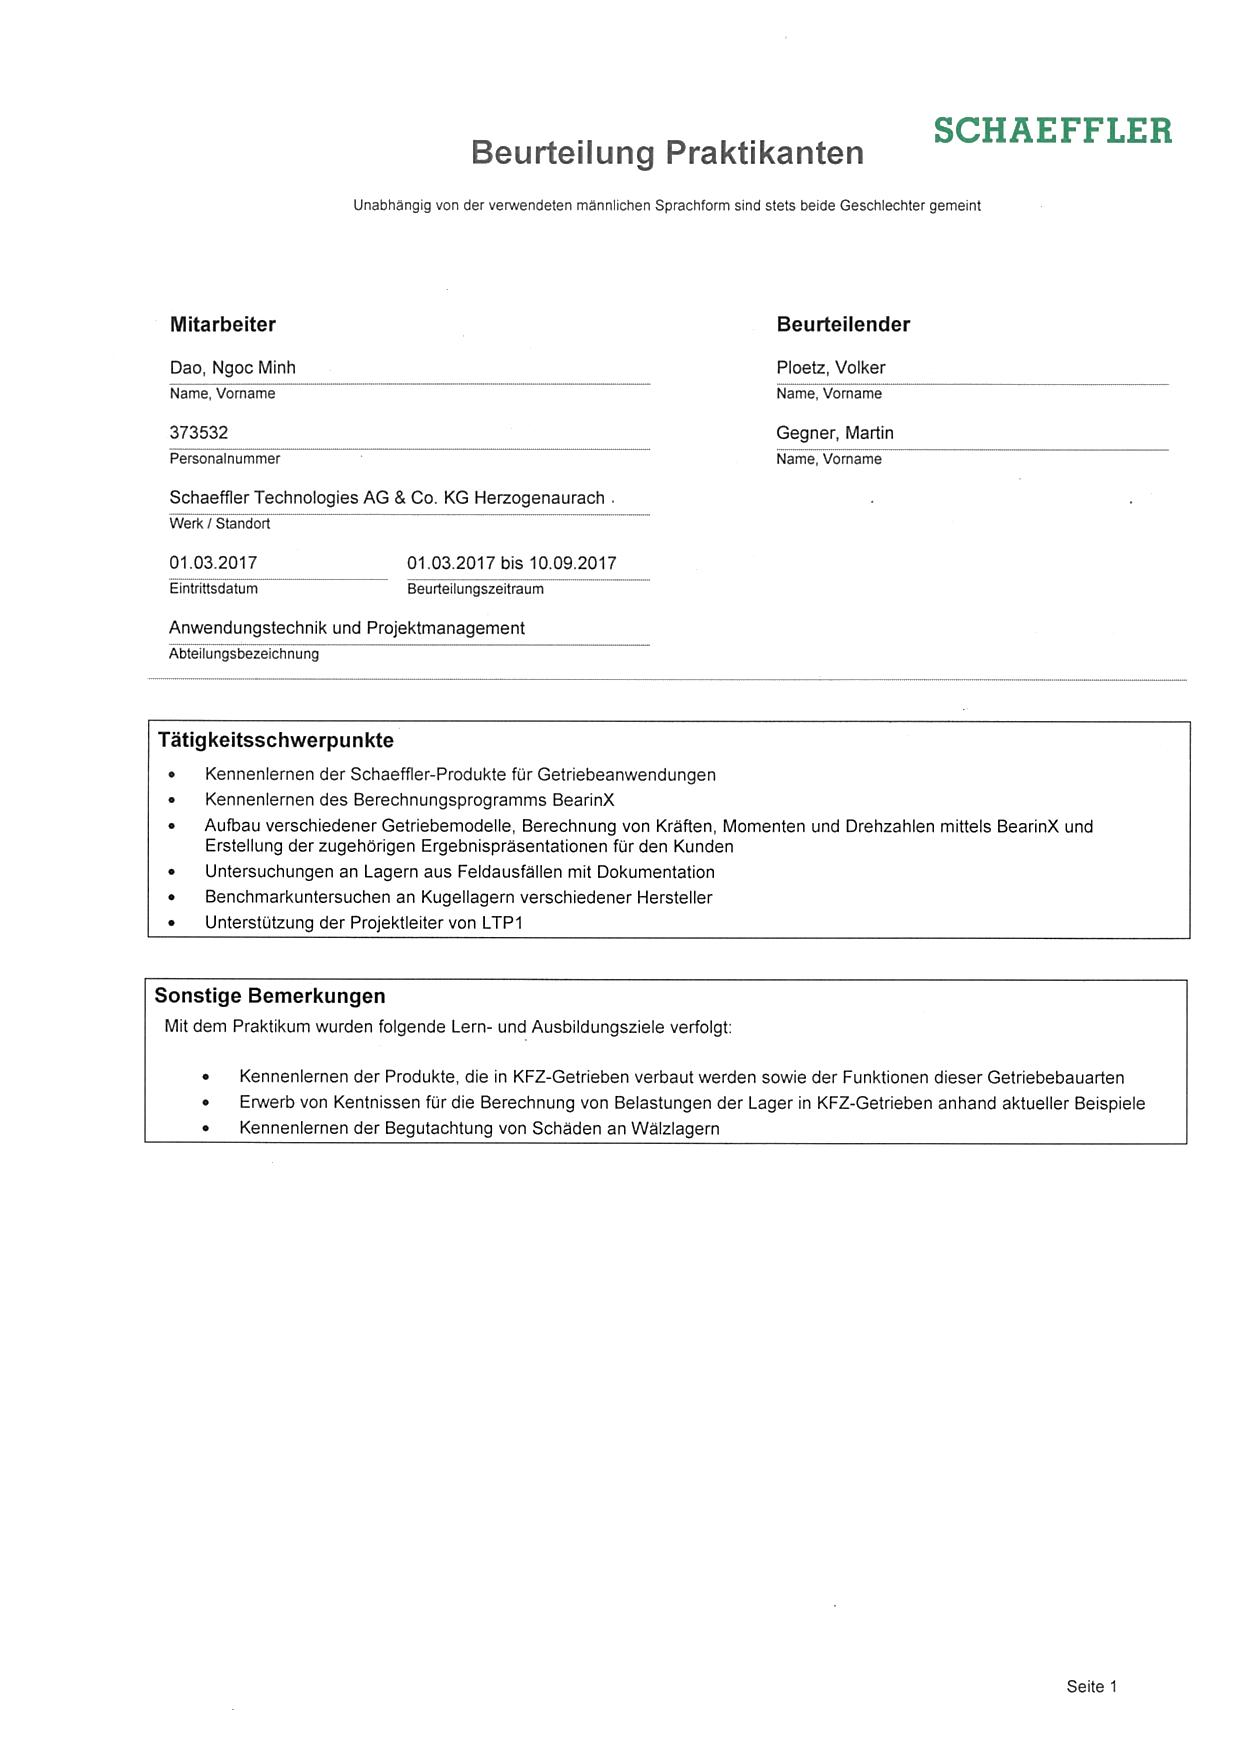
\includegraphics[width=\linewidth, keepaspectratio]{./zeugnisse/praktikumzeugnis_1.jpg}
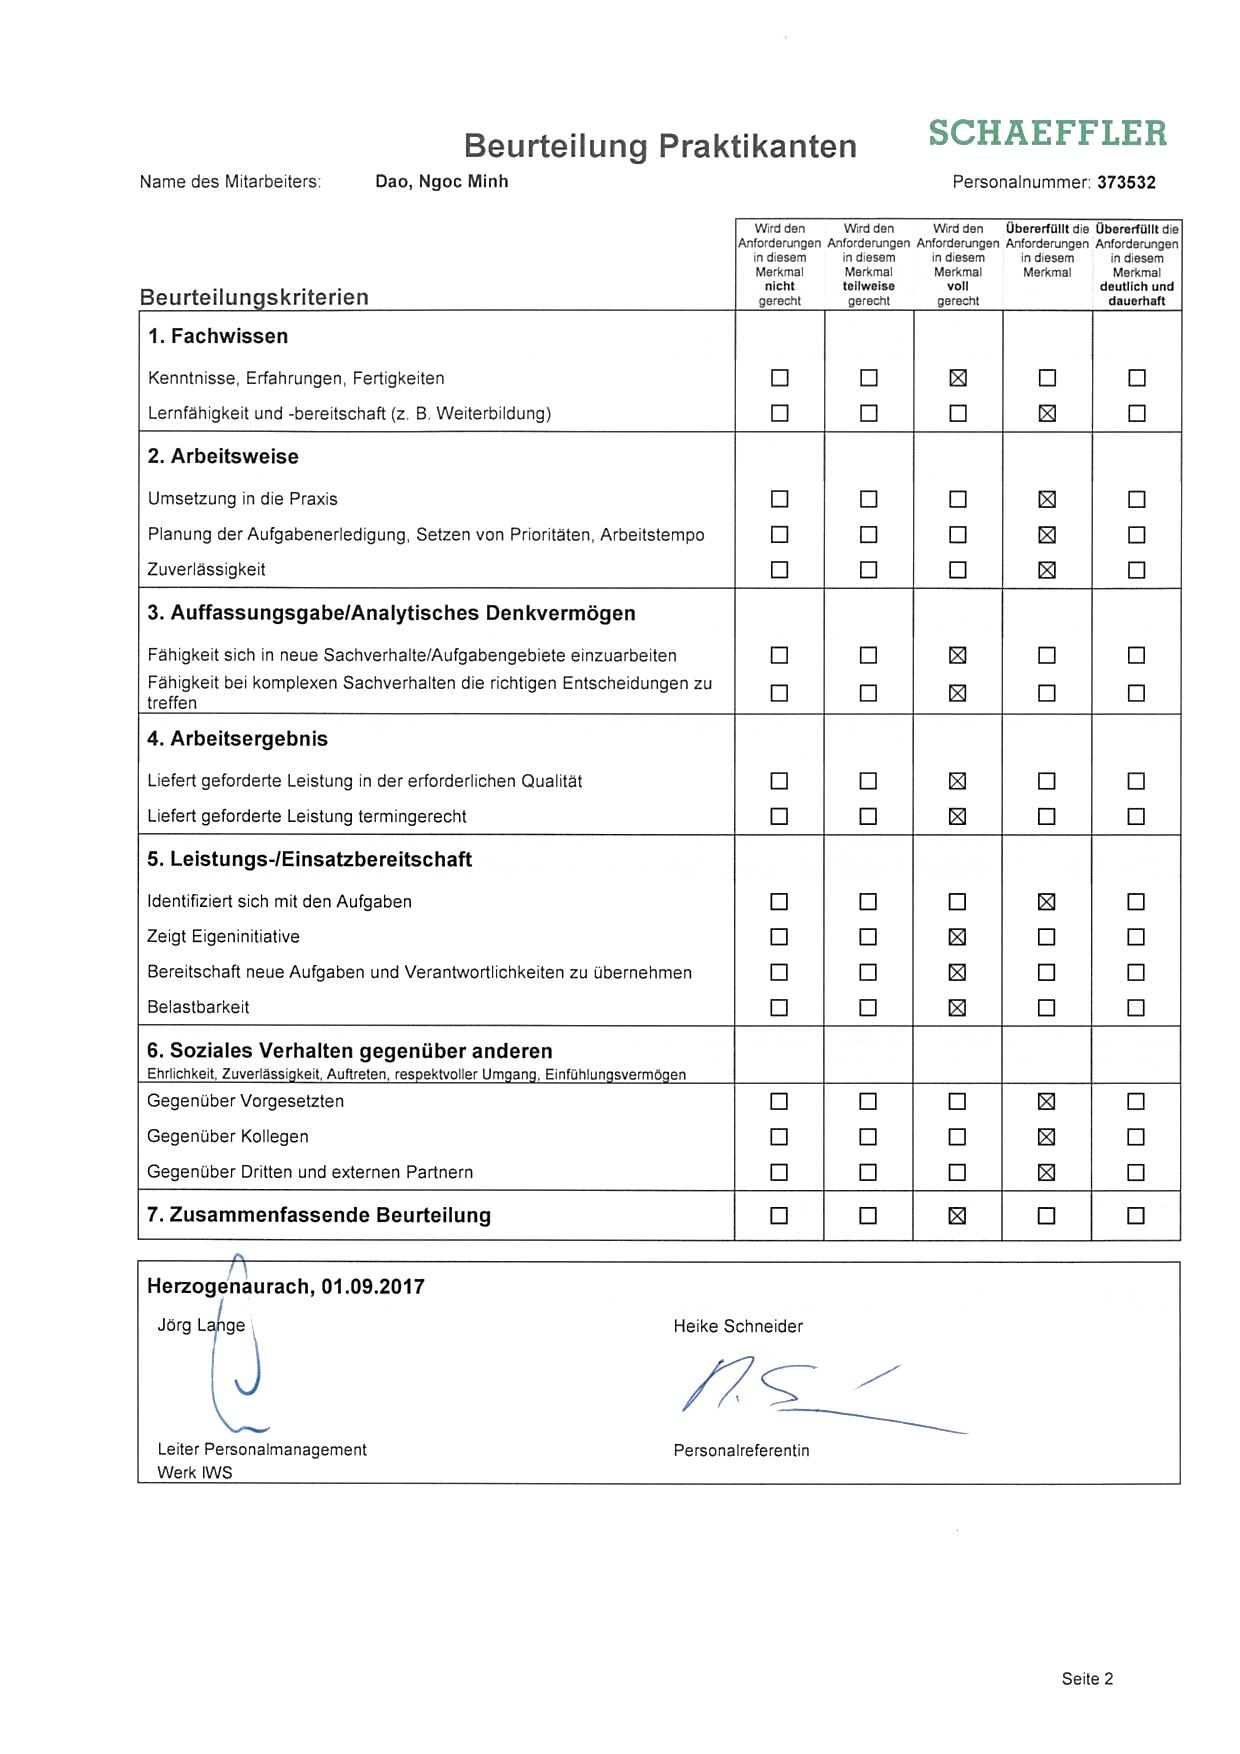
\includegraphics[width=\linewidth, keepaspectratio]{./zeugnisse/praktikumzeugnis_2.jpg}

\newpage
\bookmark[page=\thepage, level=0]{Masterzeugnis}
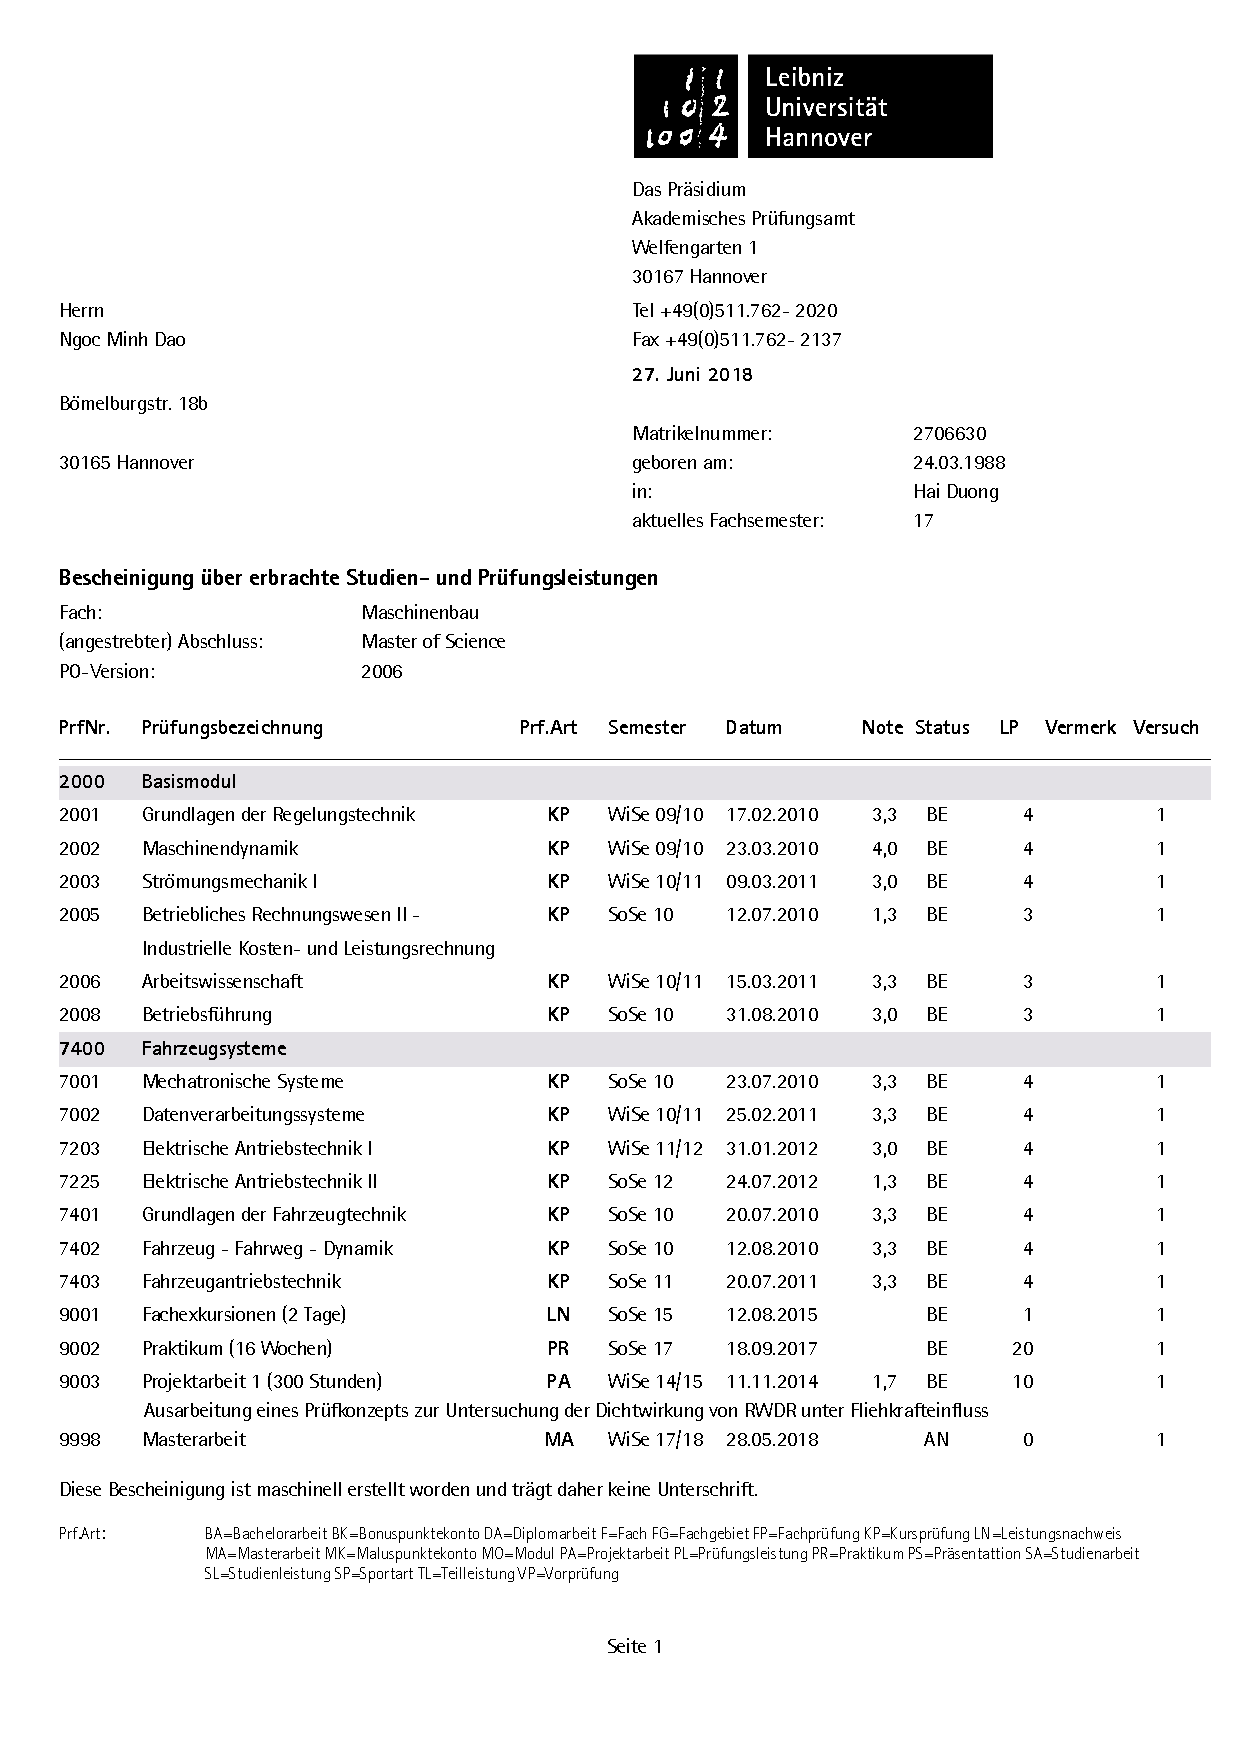
\includepdf[pages=-1]{./zeugnisse/luh_noten.pdf}

%\newpage
%\bookmark[page=\thepage, level=0]{Bachelorurkunde}
%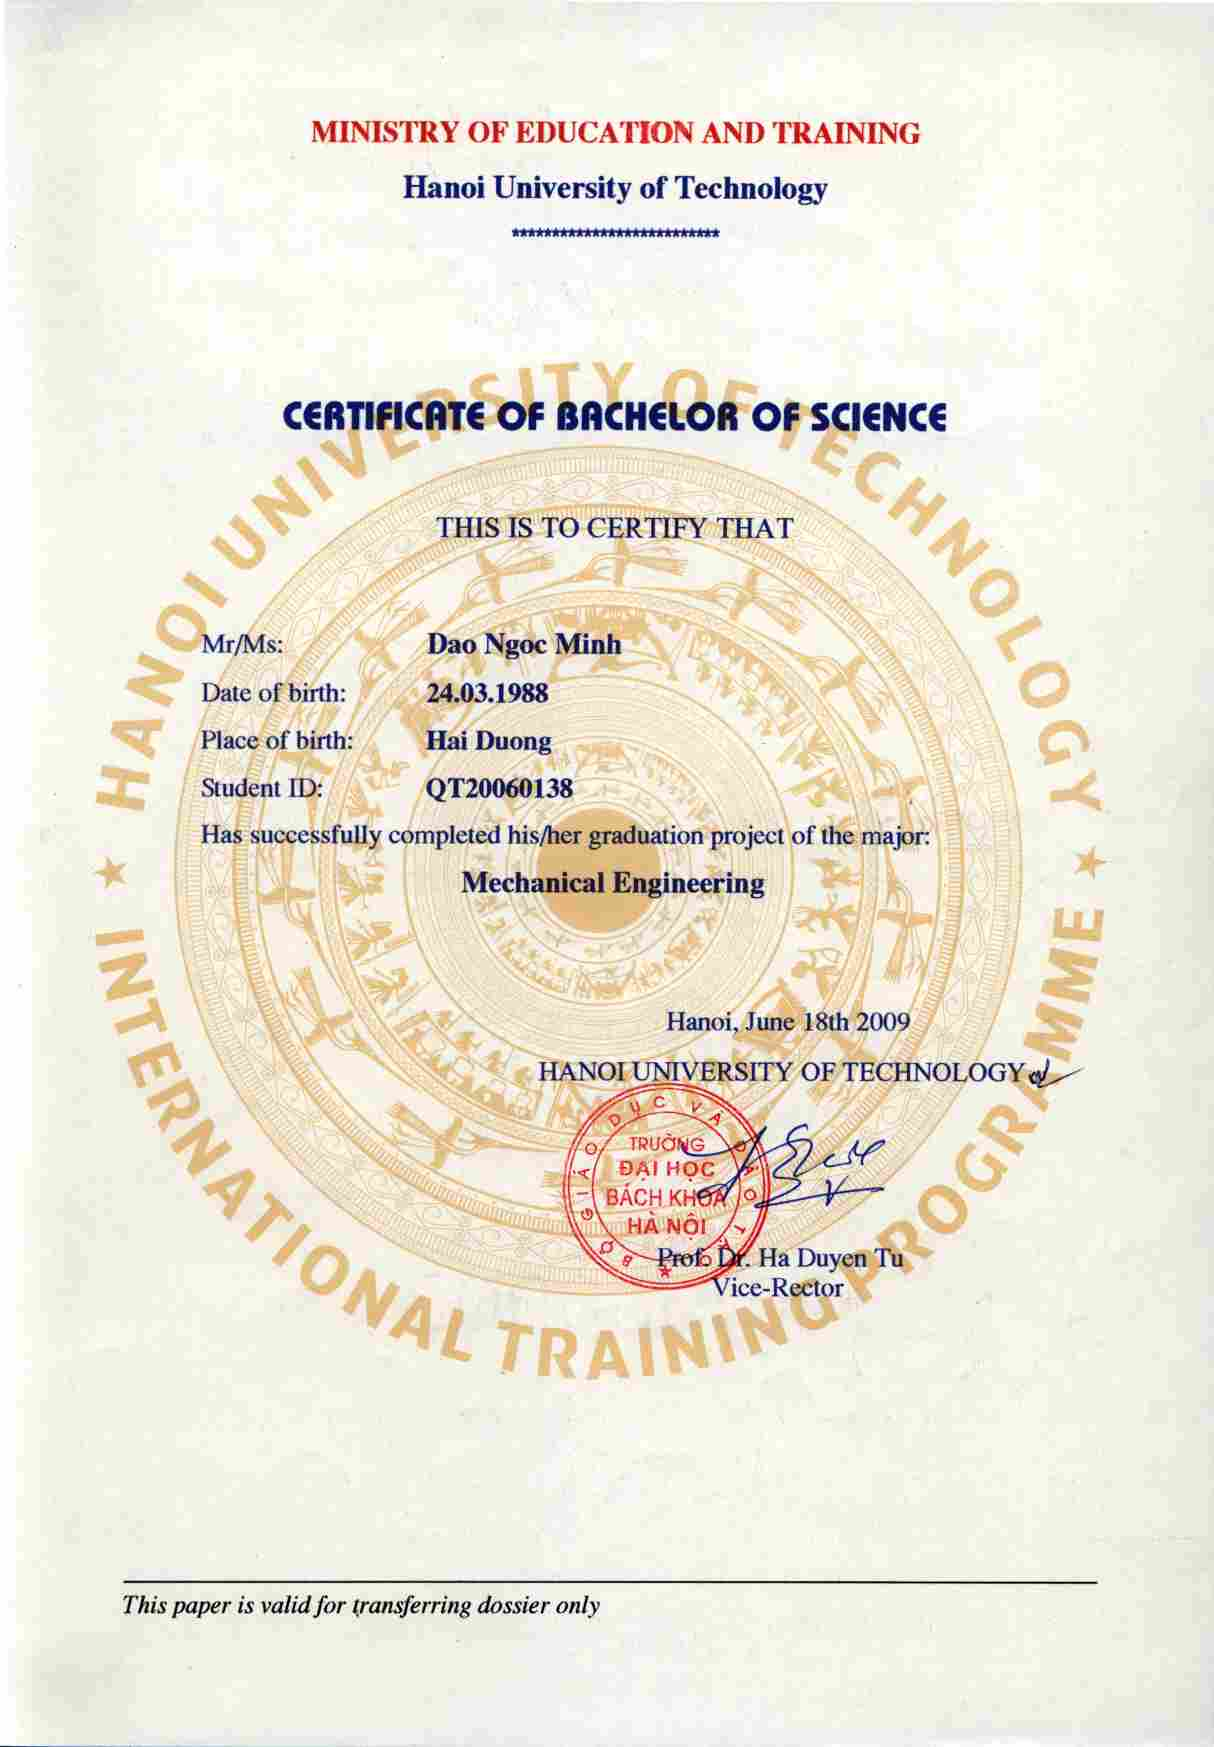
\includegraphics [width=\linewidth, height=\textheight] {./zeugnisse/hust_bachelor_lq.jpg}

\newpage
\bookmark[page=\thepage, level=0]{Bachelorzeugnisse}
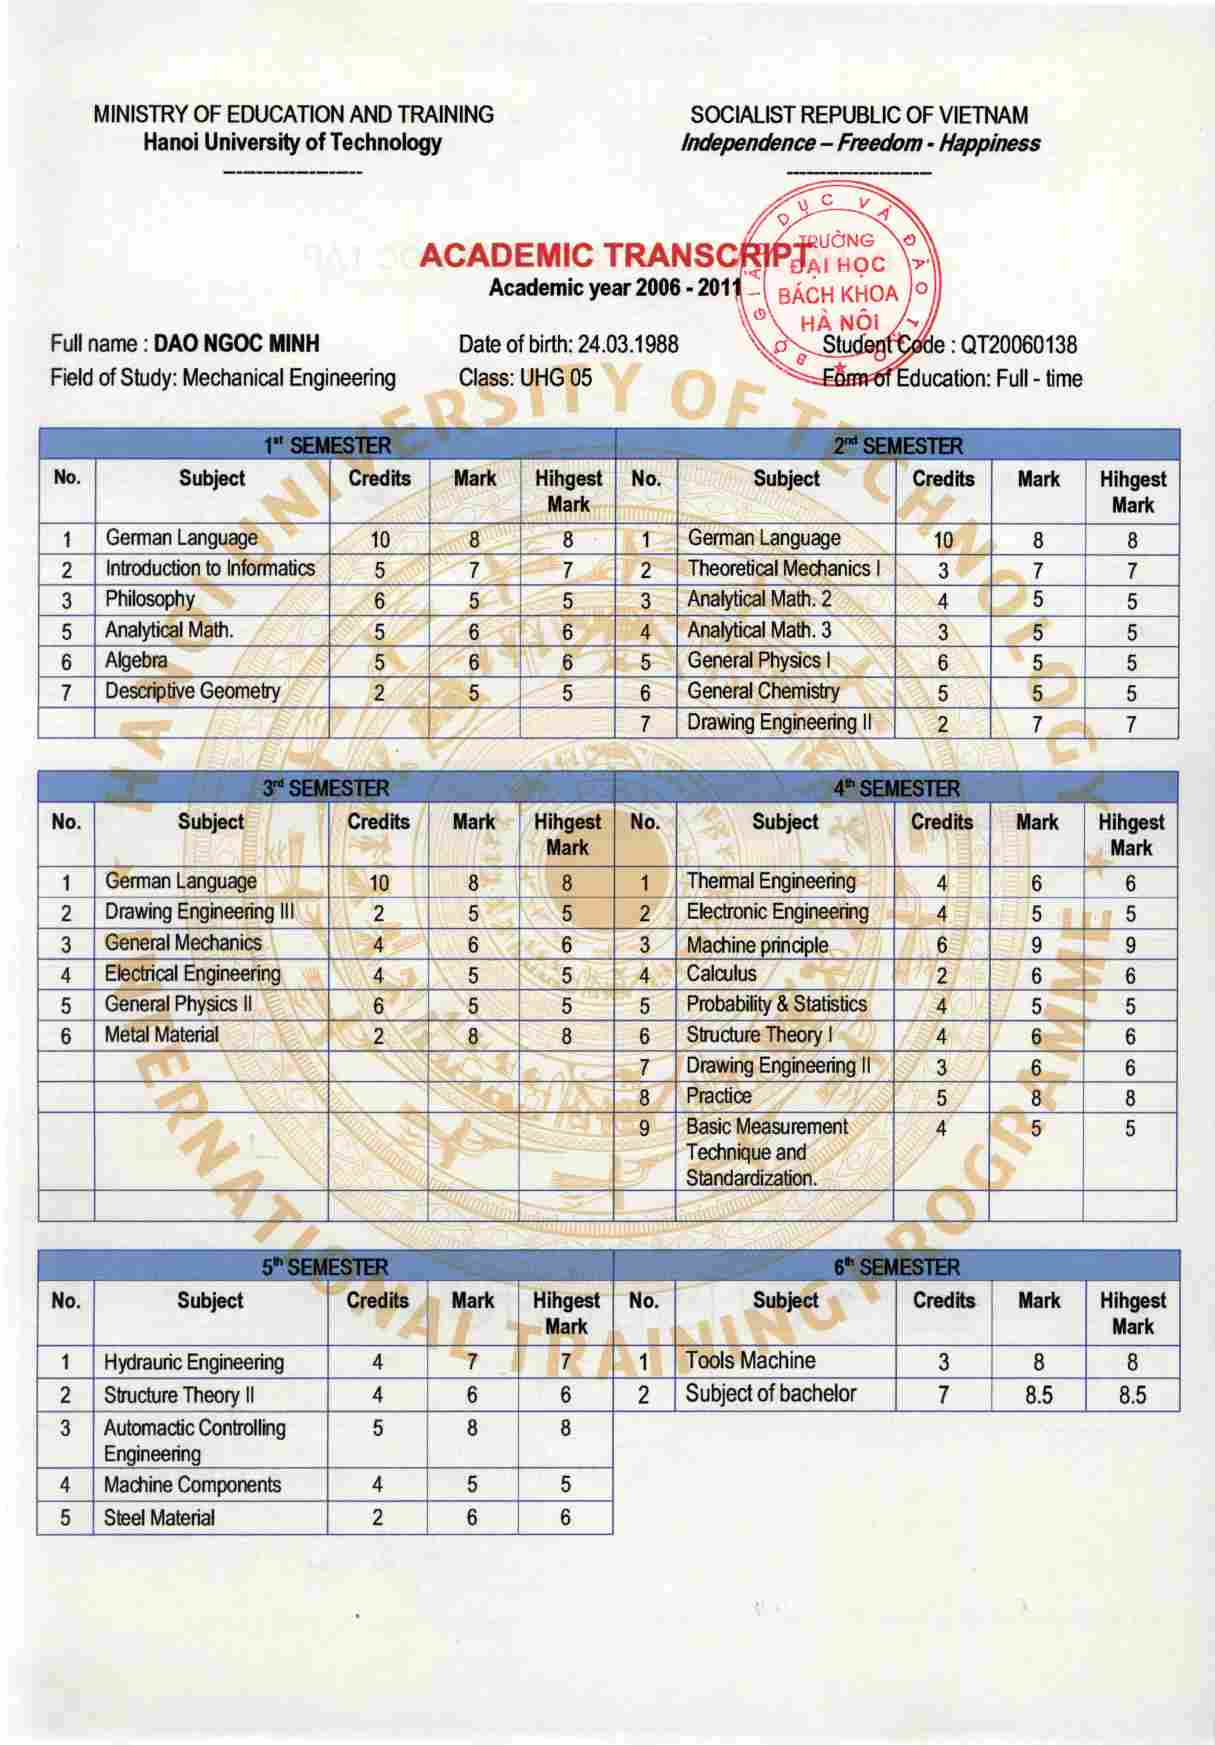
\includegraphics [width=\linewidth, height=\textheight] {./zeugnisse/hust_bachelor_noten_eng_lq.jpg}% }}}

% Bescheinigungen {{{
\newpage
\bookmark[page=\thepage, level=-1]{Bescheinigungen}

% CAD/CAE {{{
\newpage
\bookmark[page=\thepage, level=0]{CAD/CAE}

% ----------------------------------------
% Multisoft Virtual Academy - PTC Creo
% ----------------------------------------
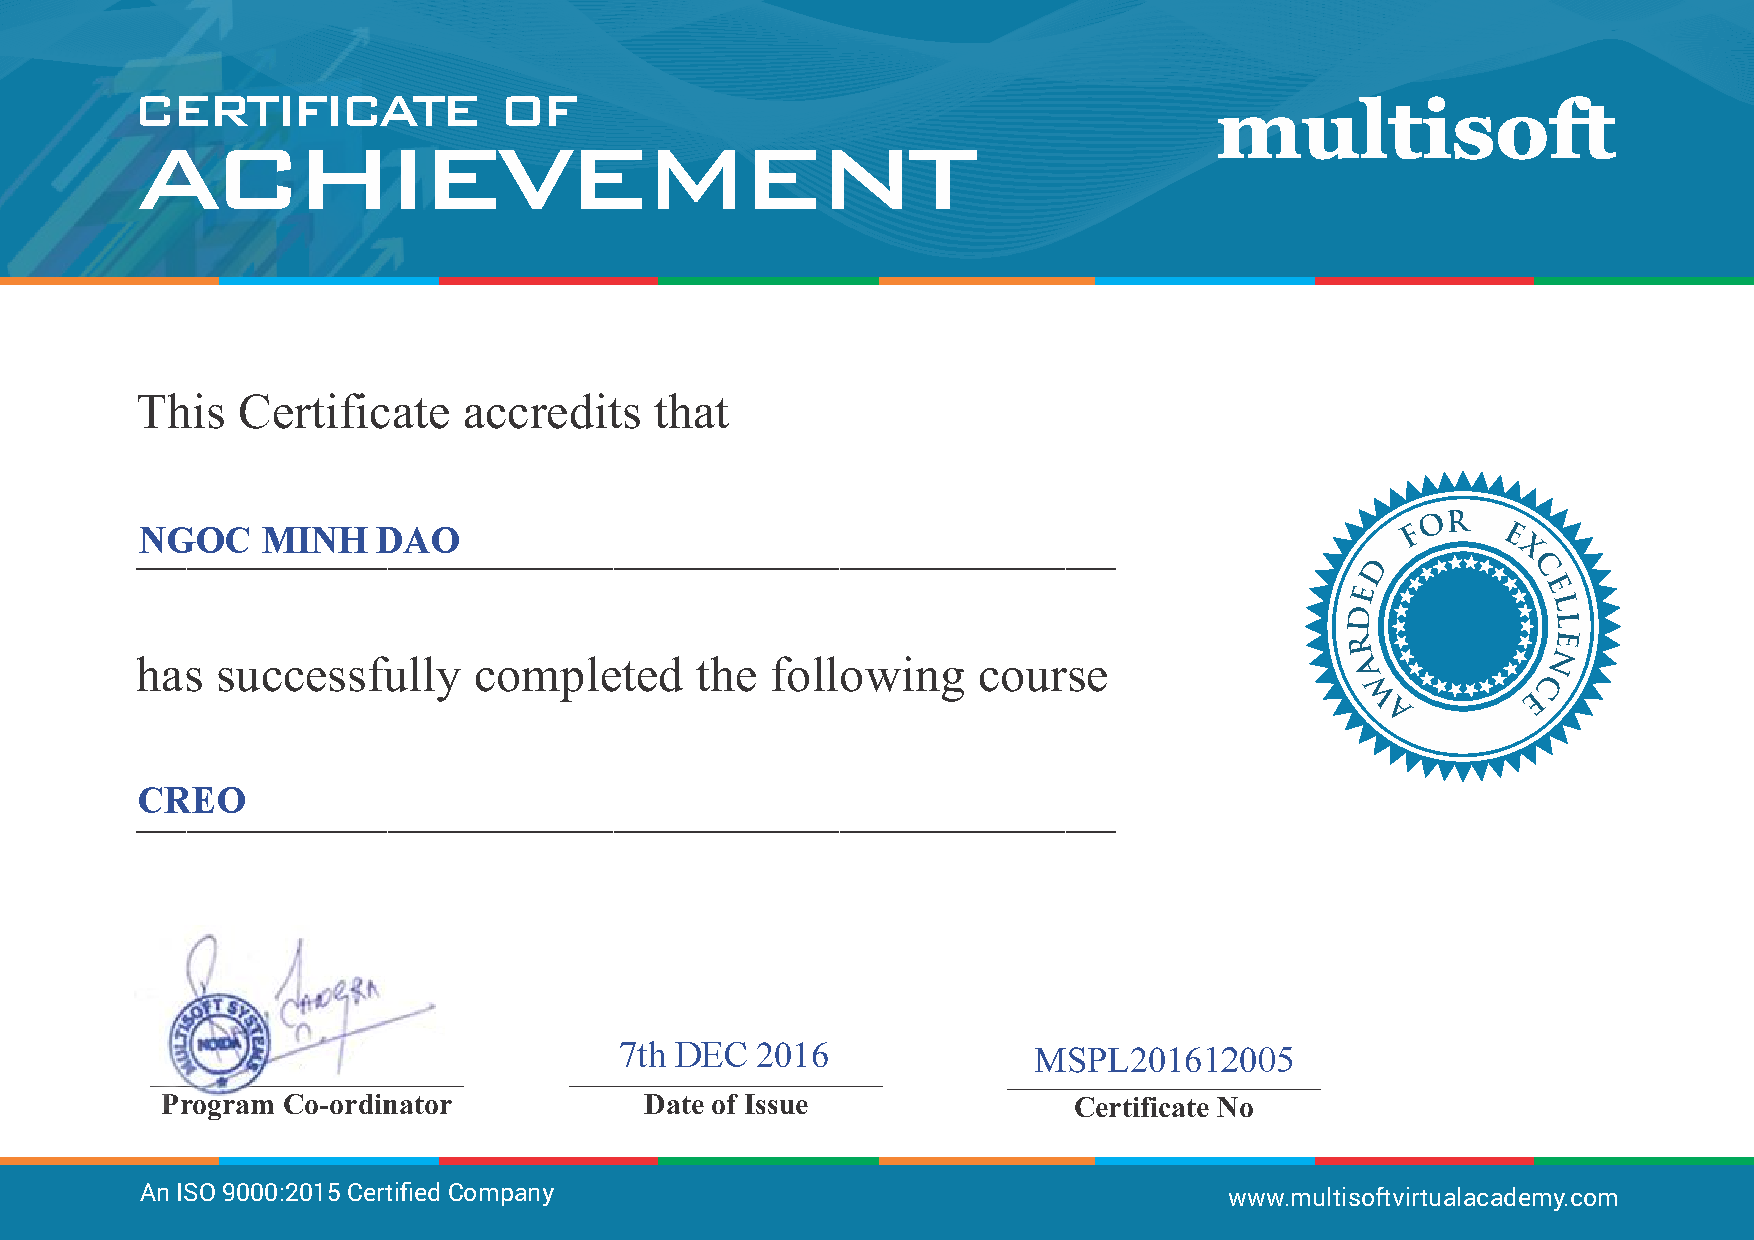
\includepdf [angle=90, pages=-1] {./zeugnisse/creo.pdf}

% ----------------------------------------
% Christiani Akademie - CAD Kompakt
% ----------------------------------------
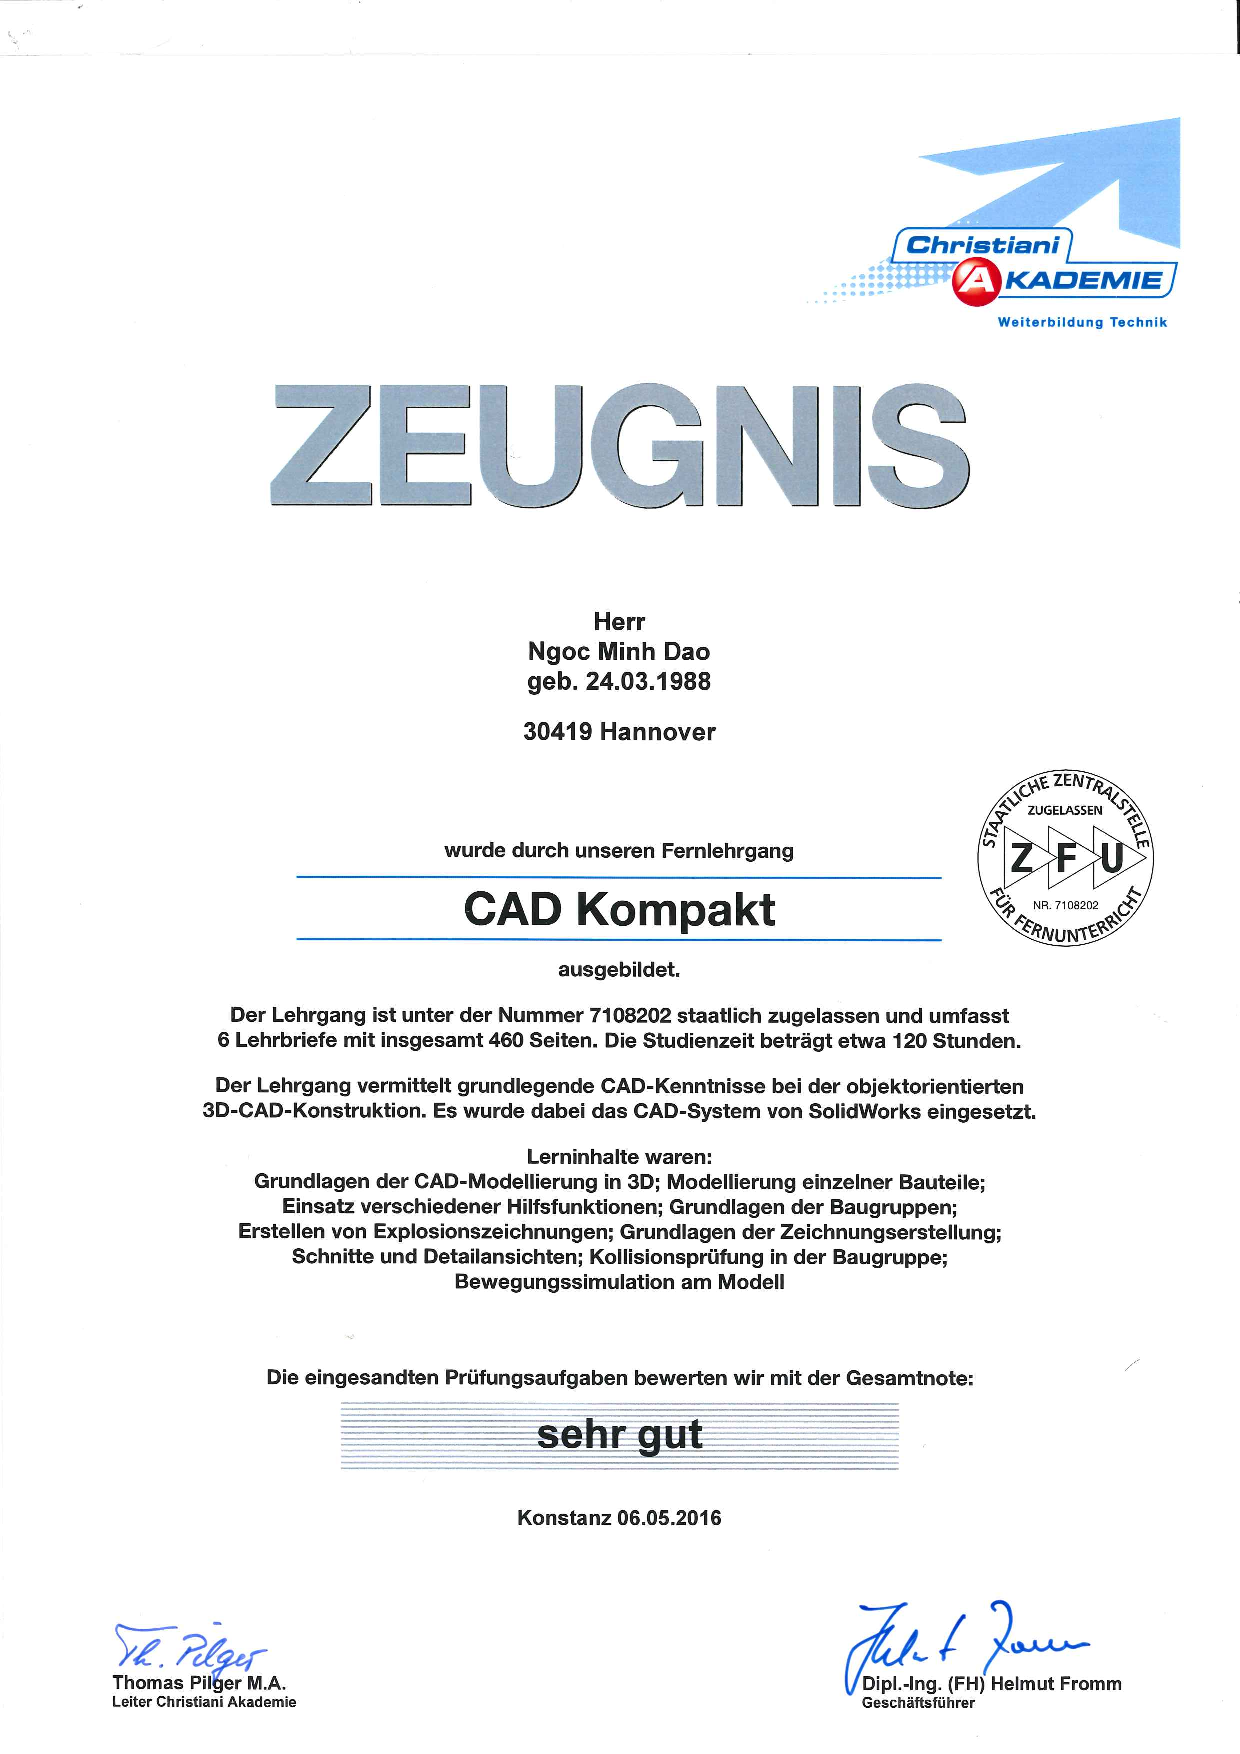
\includepdf [landscape=false, pages=-1] {./zeugnisse/christiani_akademie_cad-kompakt.pdf}

% ----------------------------------------
% Ipeg - Autodesk Inventor
% ----------------------------------------
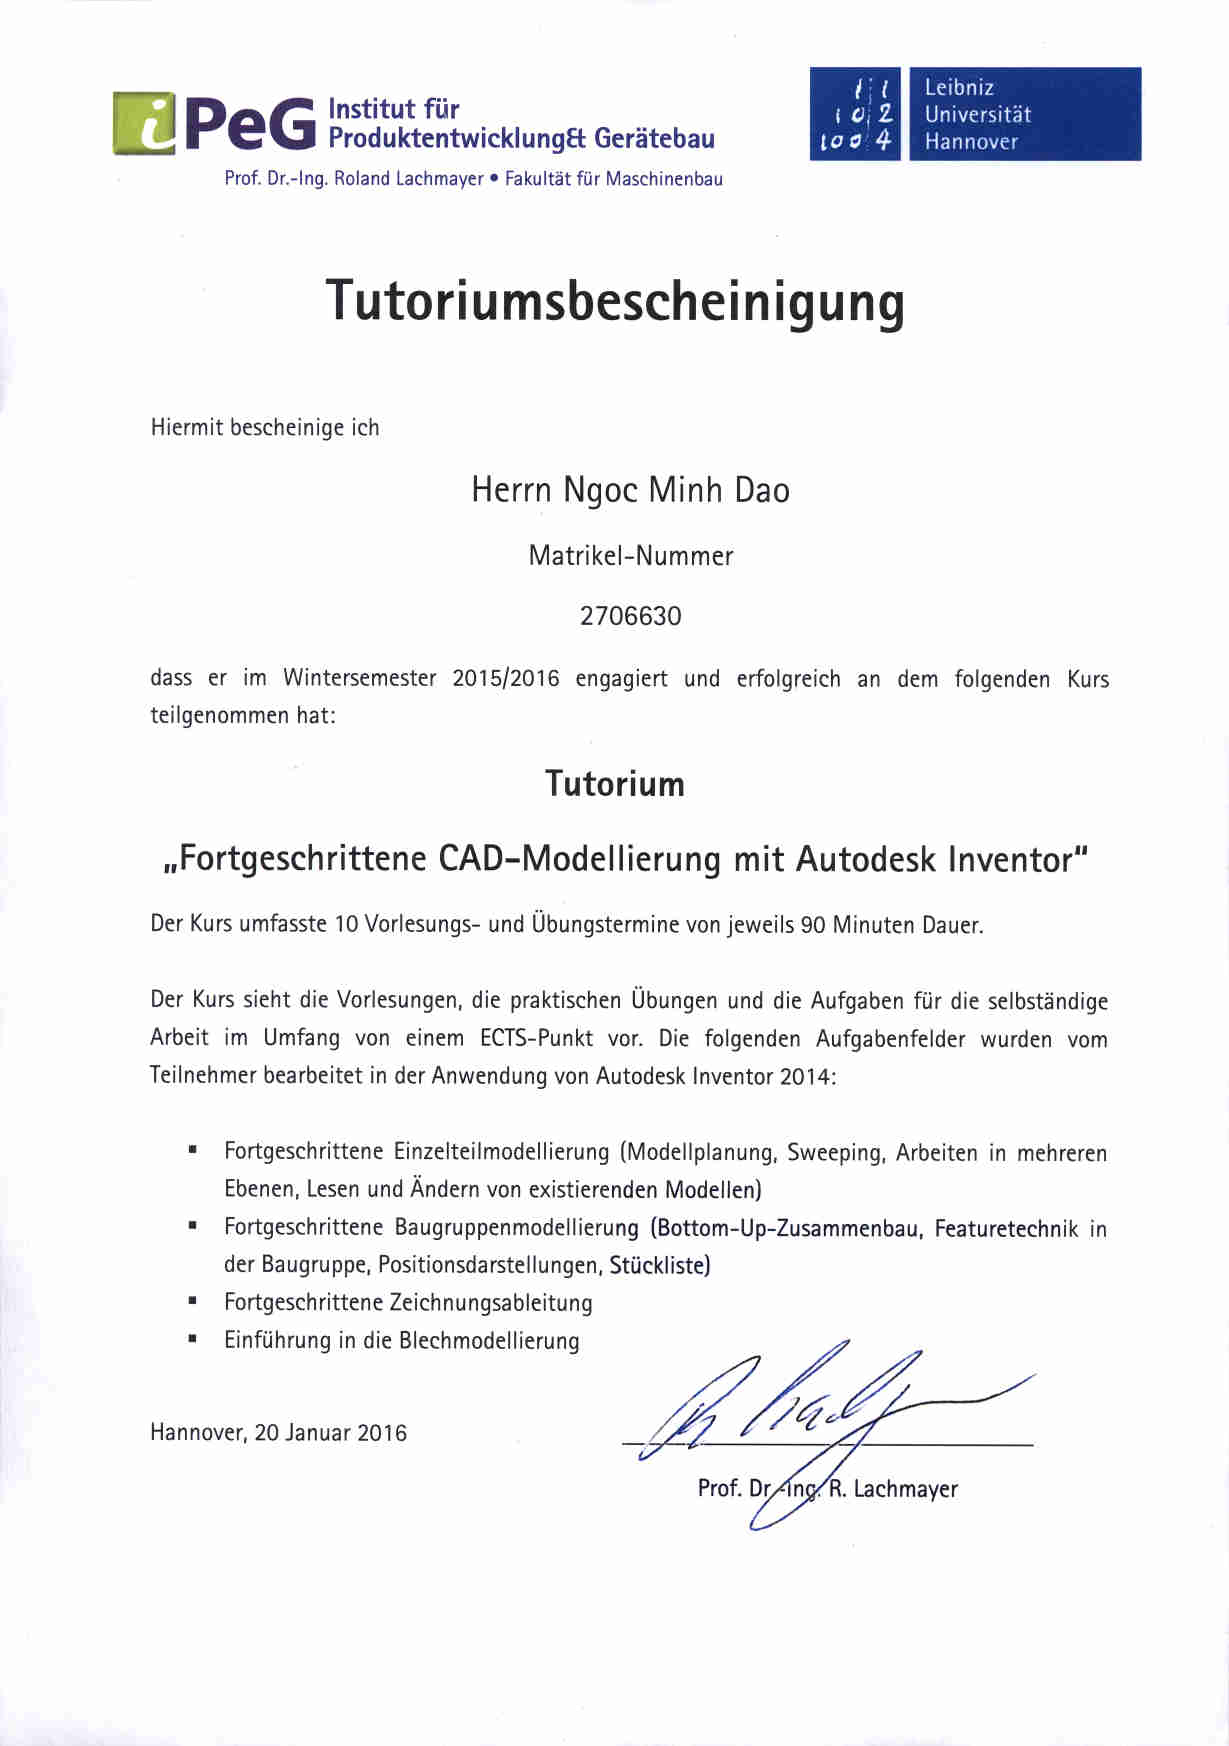
\includegraphics [width=\linewidth, height=\textheight] {./zeugnisse/ipeg_autodesk_inventor_lq.jpg}


% ----------------------------------------
% ITA - Autodesk Inventor
% ----------------------------------------
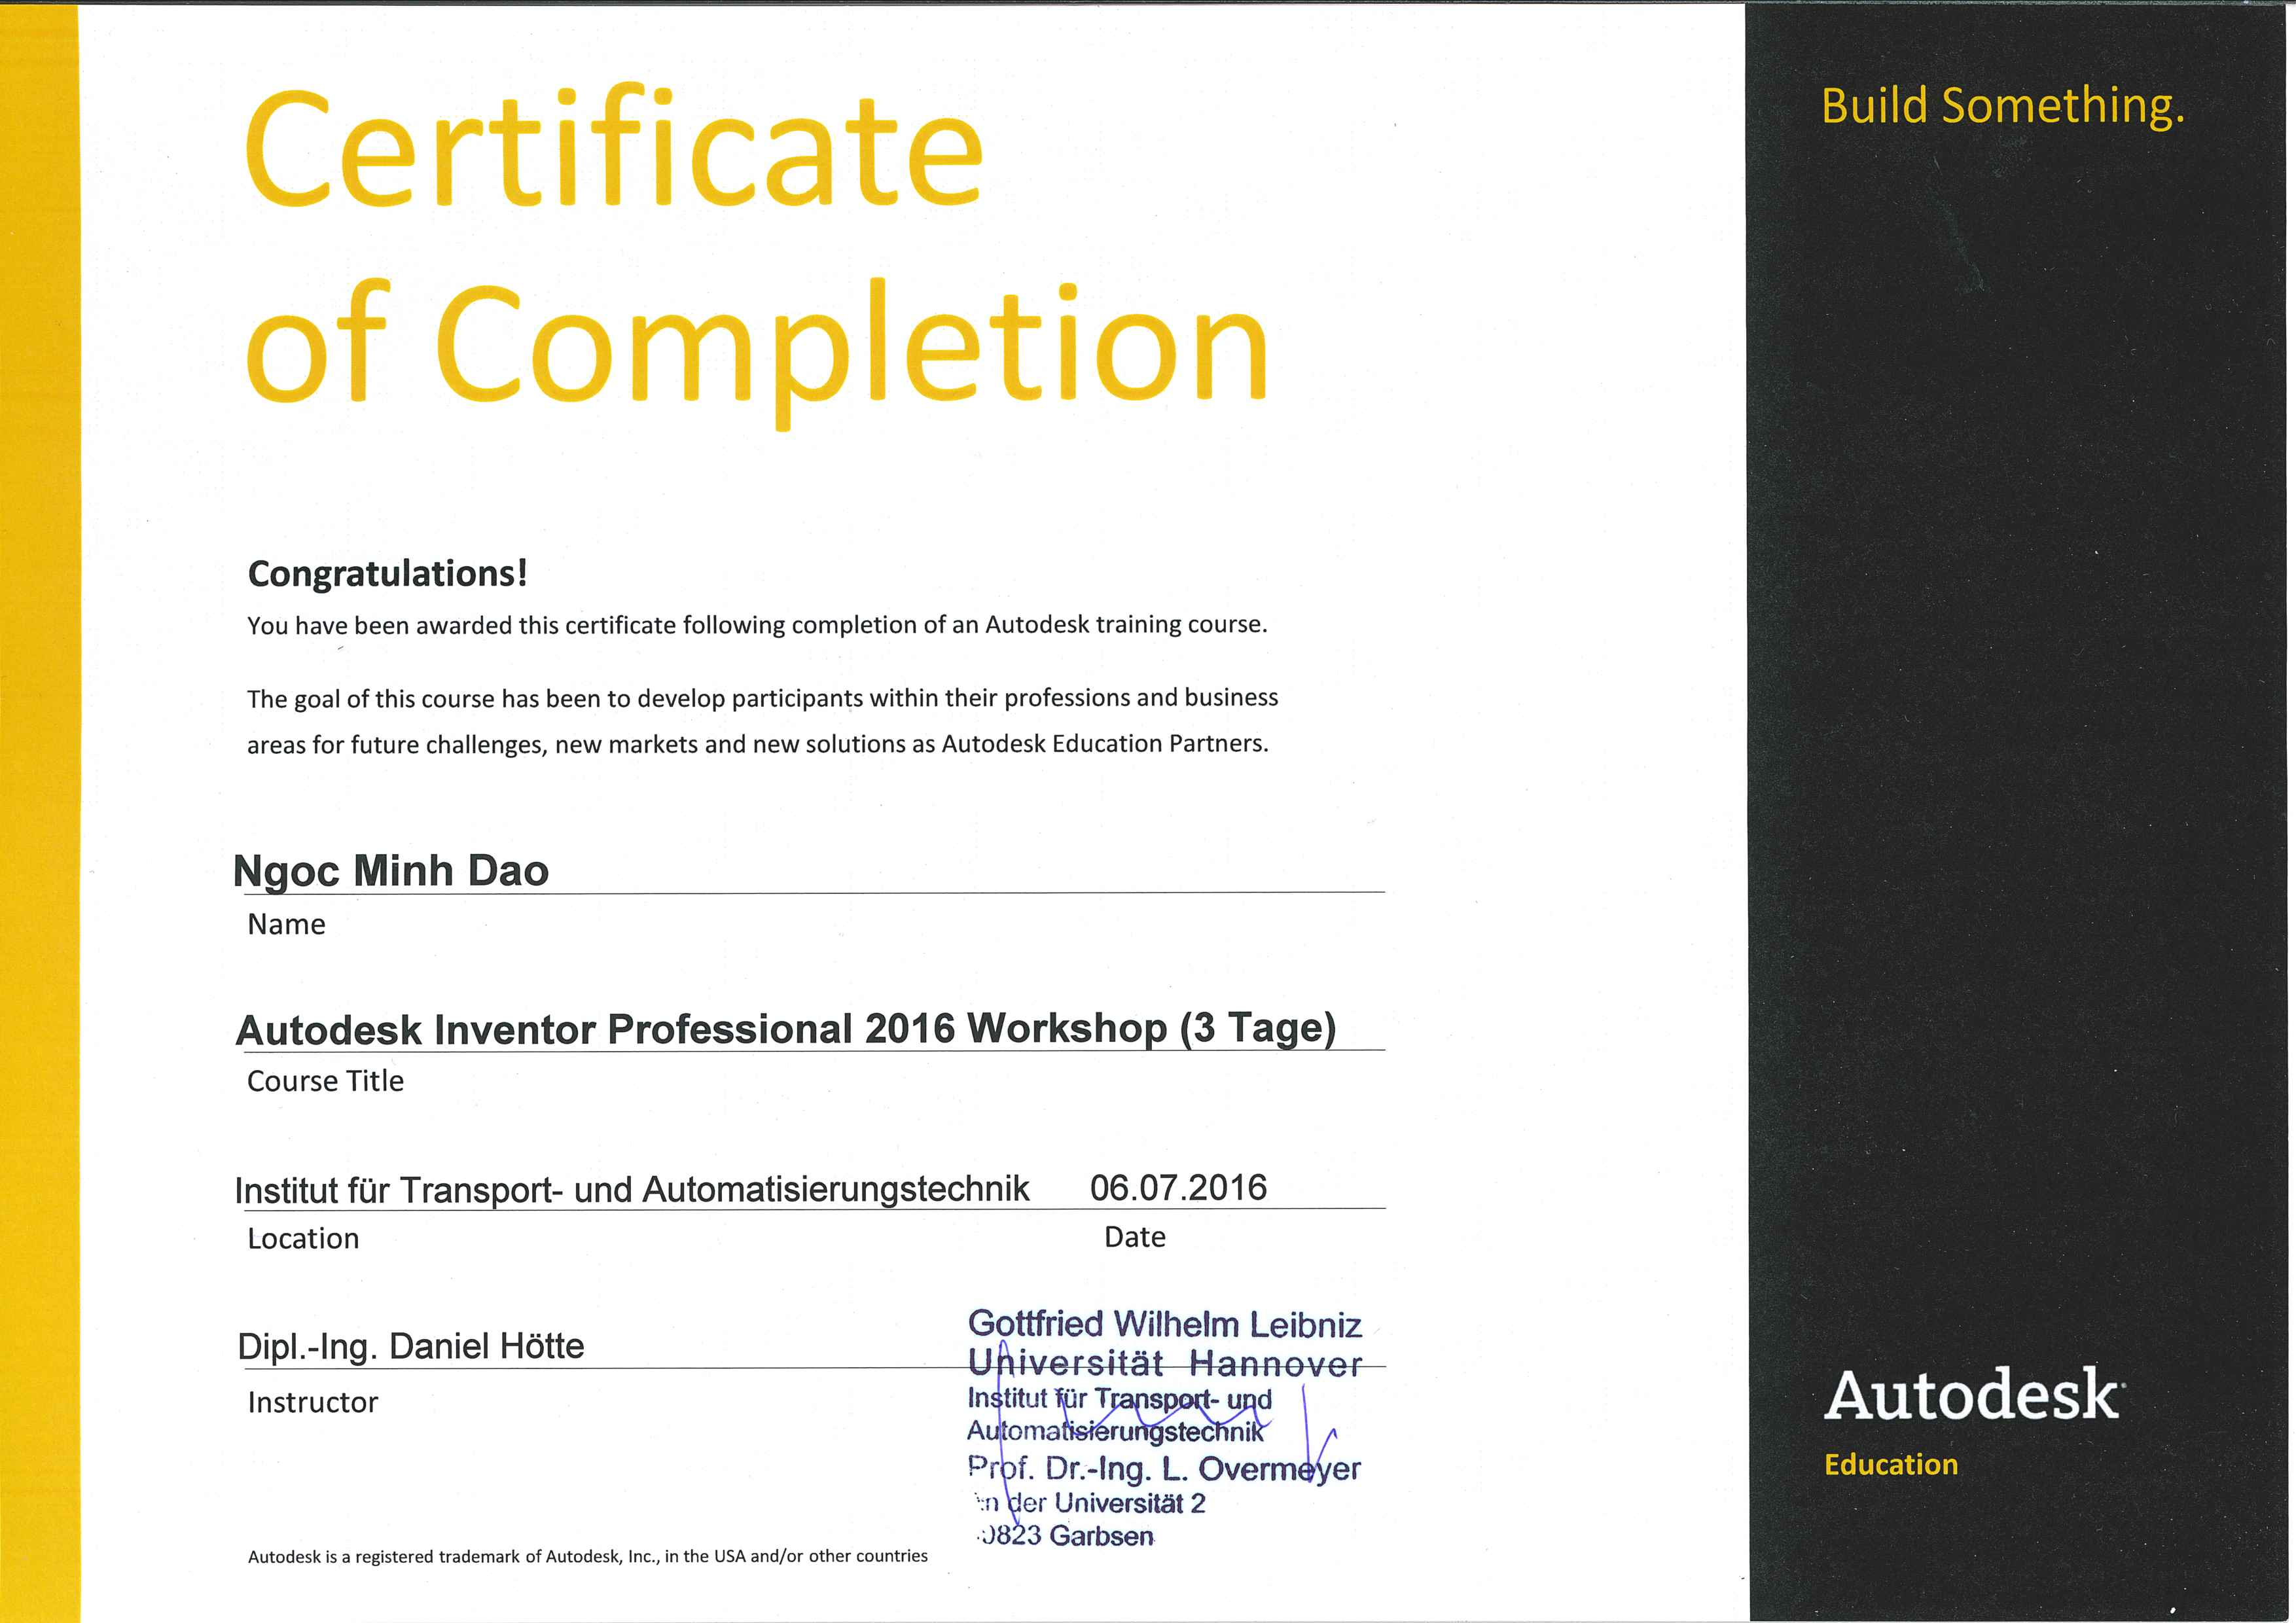
\includegraphics [angle=90 ,width=\linewidth, height=\textheight] {./zeugnisse/ita_inventor.jpg}


% ----------------------------------------
% IDS - Ansys Workbench
% ----------------------------------------
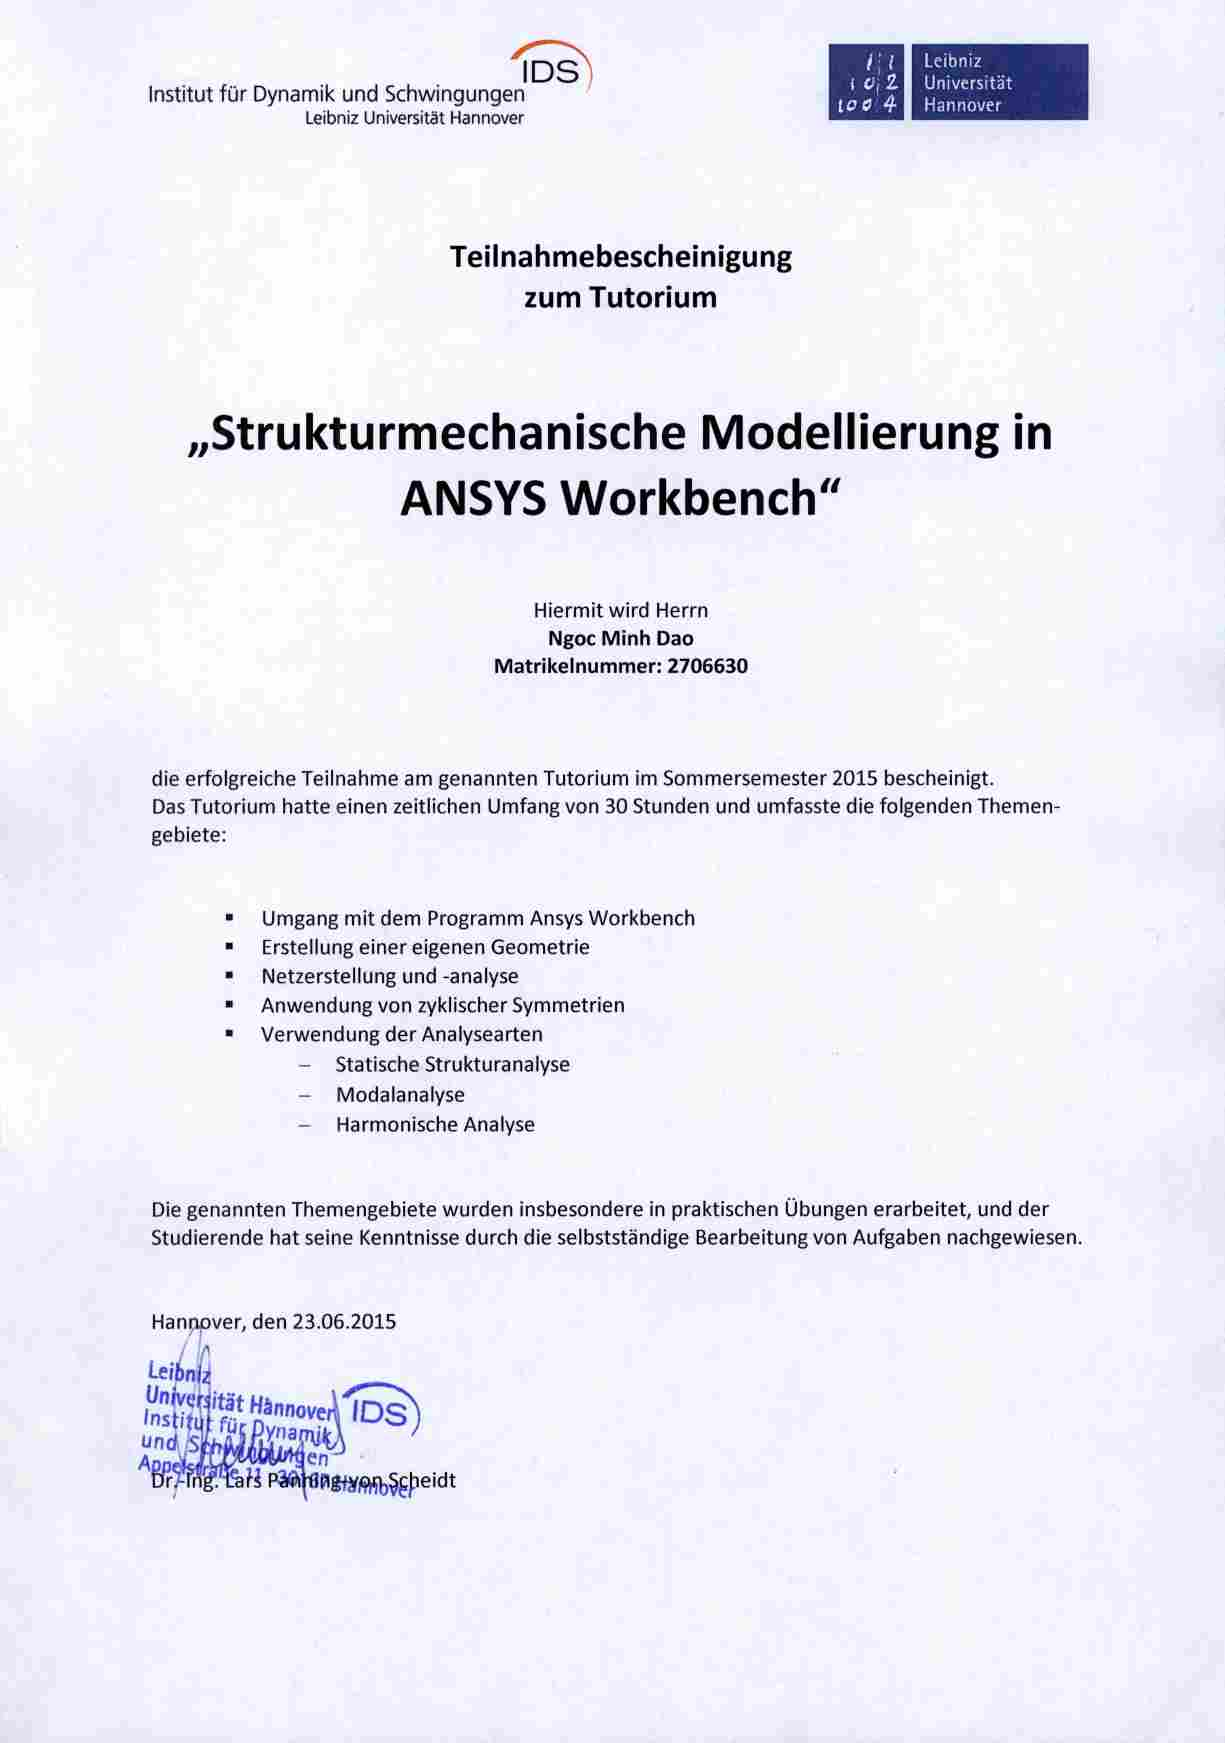
\includegraphics [width=\linewidth, height=\textheight] {./zeugnisse/ids_ansys_workbench_lq.jpg}

% ----------------------------------------
% ITV - CFD in der Verbrennungstechnik
% ----------------------------------------
%\newpage
%\includegraphics[width=\linewidth, height=\textheight]
%{./zeugnisse/itv_cfd_in_der_verbrennungstechnik_lq.jpg}% }}}

% Elektronik {{{
%\newpage
%\bookmark[page=\thepage, level=0]{Elektronik}

% ----------------------------------------
% University Texas UT603x - Embedded Systems - Shape the World
% ----------------------------------------
%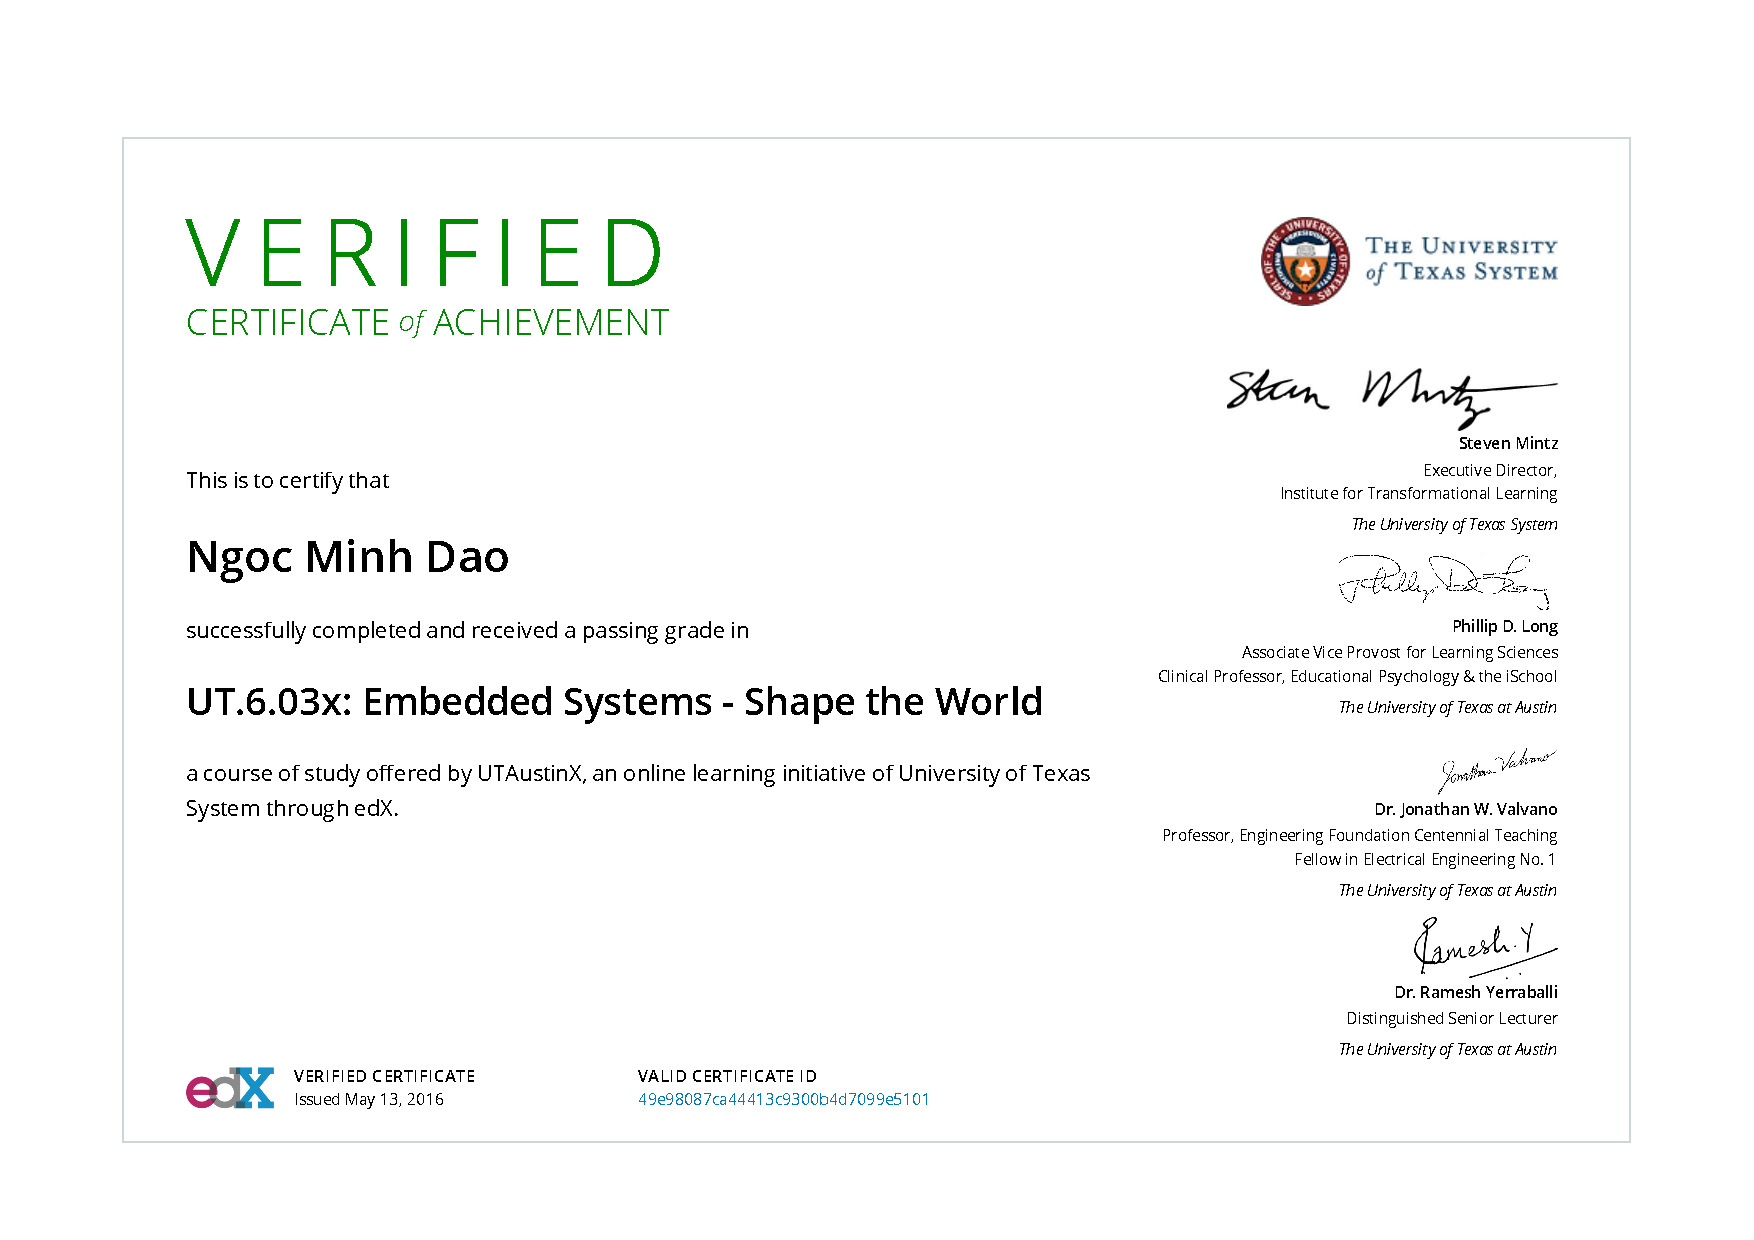
\includepdf [angle=90, pages=-1] {./zeugnisse/utaustinx_ut_603x_certificate_edx.pdf}
% }}}

% Programmiersprachen {{{
\newpage
\bookmark[page=\thepage, level=0]{Programmiersprache}

% ----------------------------------------
% National Instrument - Labview
% ----------------------------------------
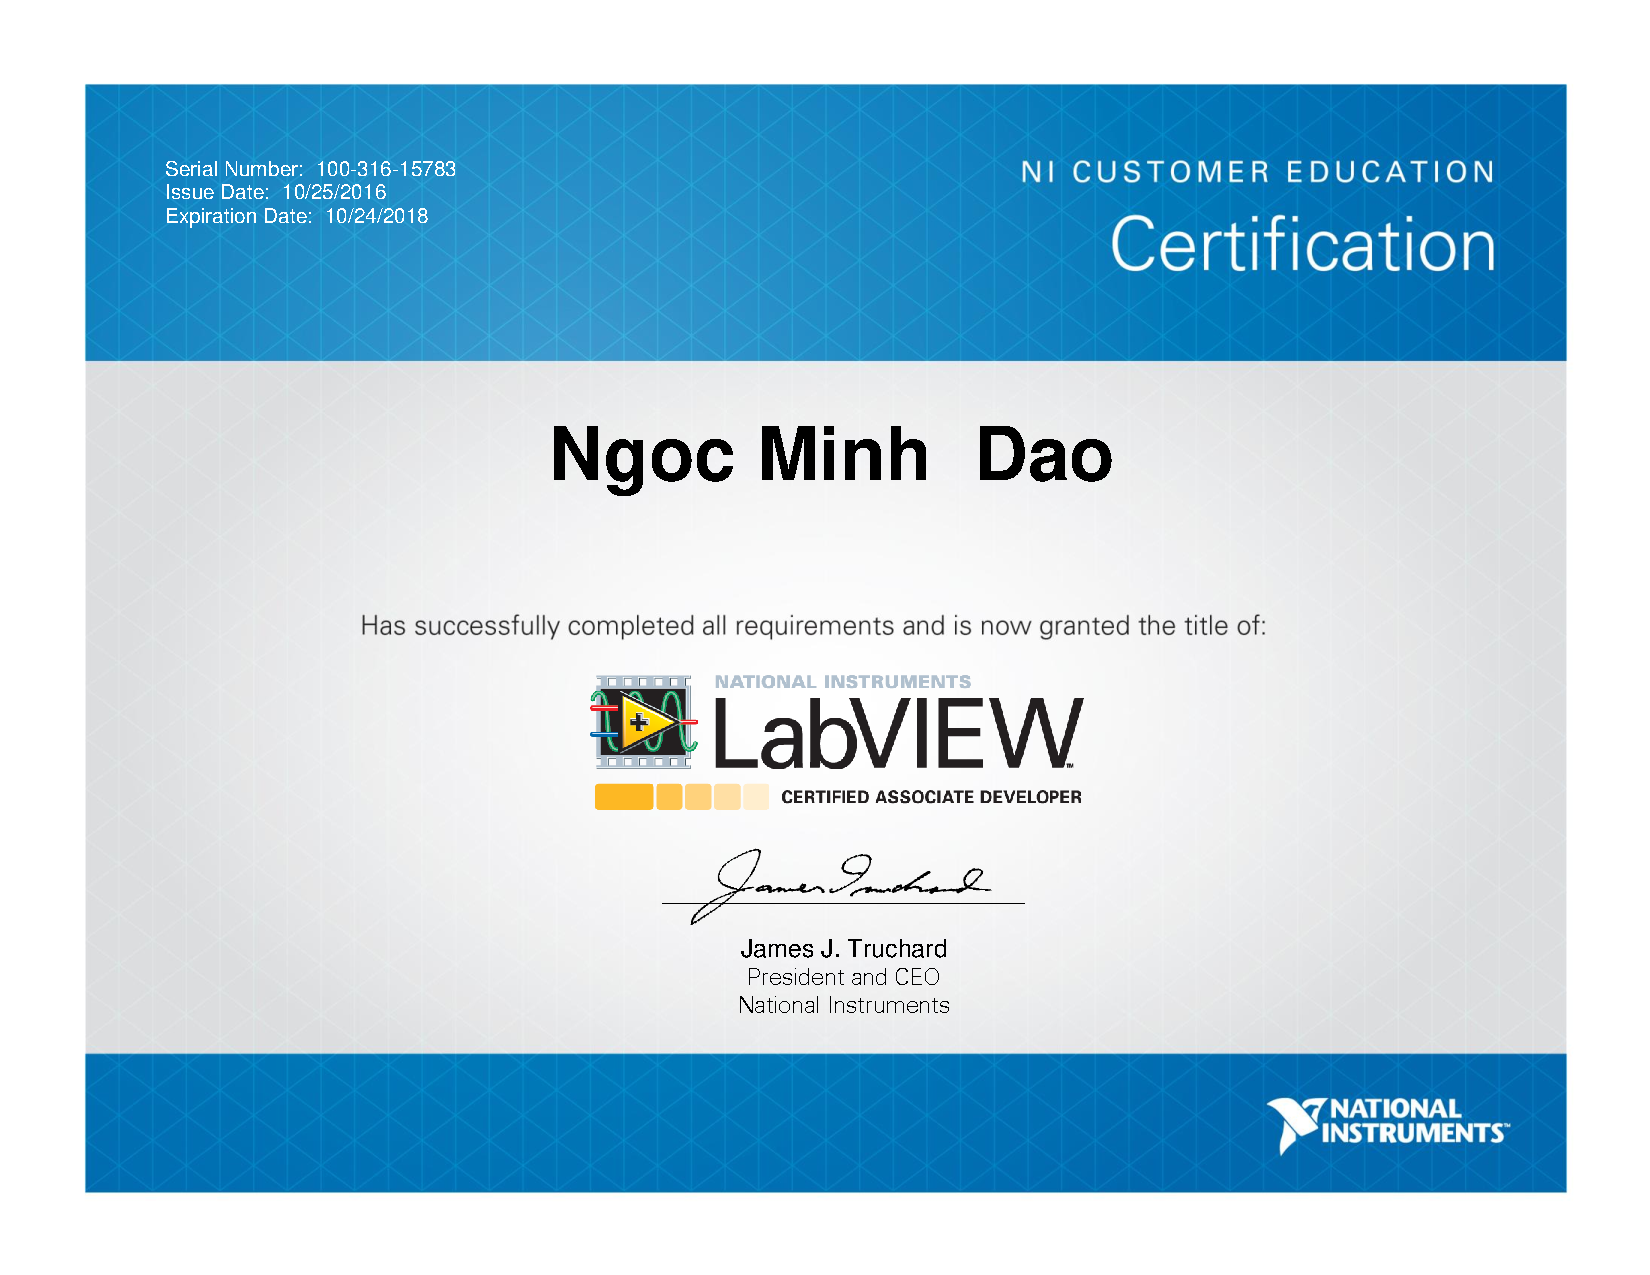
\includepdf [angle=90, pages=-1] {./zeugnisse/labview.pdf}

% ----------------------------------------
% Microsft DEV204x - Programming with C#
% ----------------------------------------
%
\includepdf [angle=90, pages=-1] {./zeugnisse/microsoft_dev204x_certificate_edx.pdf}

% ----------------------------------------
% MIT 6.00.1x - Introduction to Computer Science and Programming Using Python
% ----------------------------------------
\newpage

\includepdf [angle=90, pages=-1] {./zeugnisse/mitx_6001.pdf}

% ----------------------------------------
% Microsft DAT208x - Introduction to Python for Data Science
% ----------------------------------------
%
\includepdf [angle=90, pages=-1] {./zeugnisse/microsoft_dat208x_certificate_edx.pdf}

% ----------------------------------------
% iversity - Modelling and Simulation using MATLAB Simulink
% ----------------------------------------
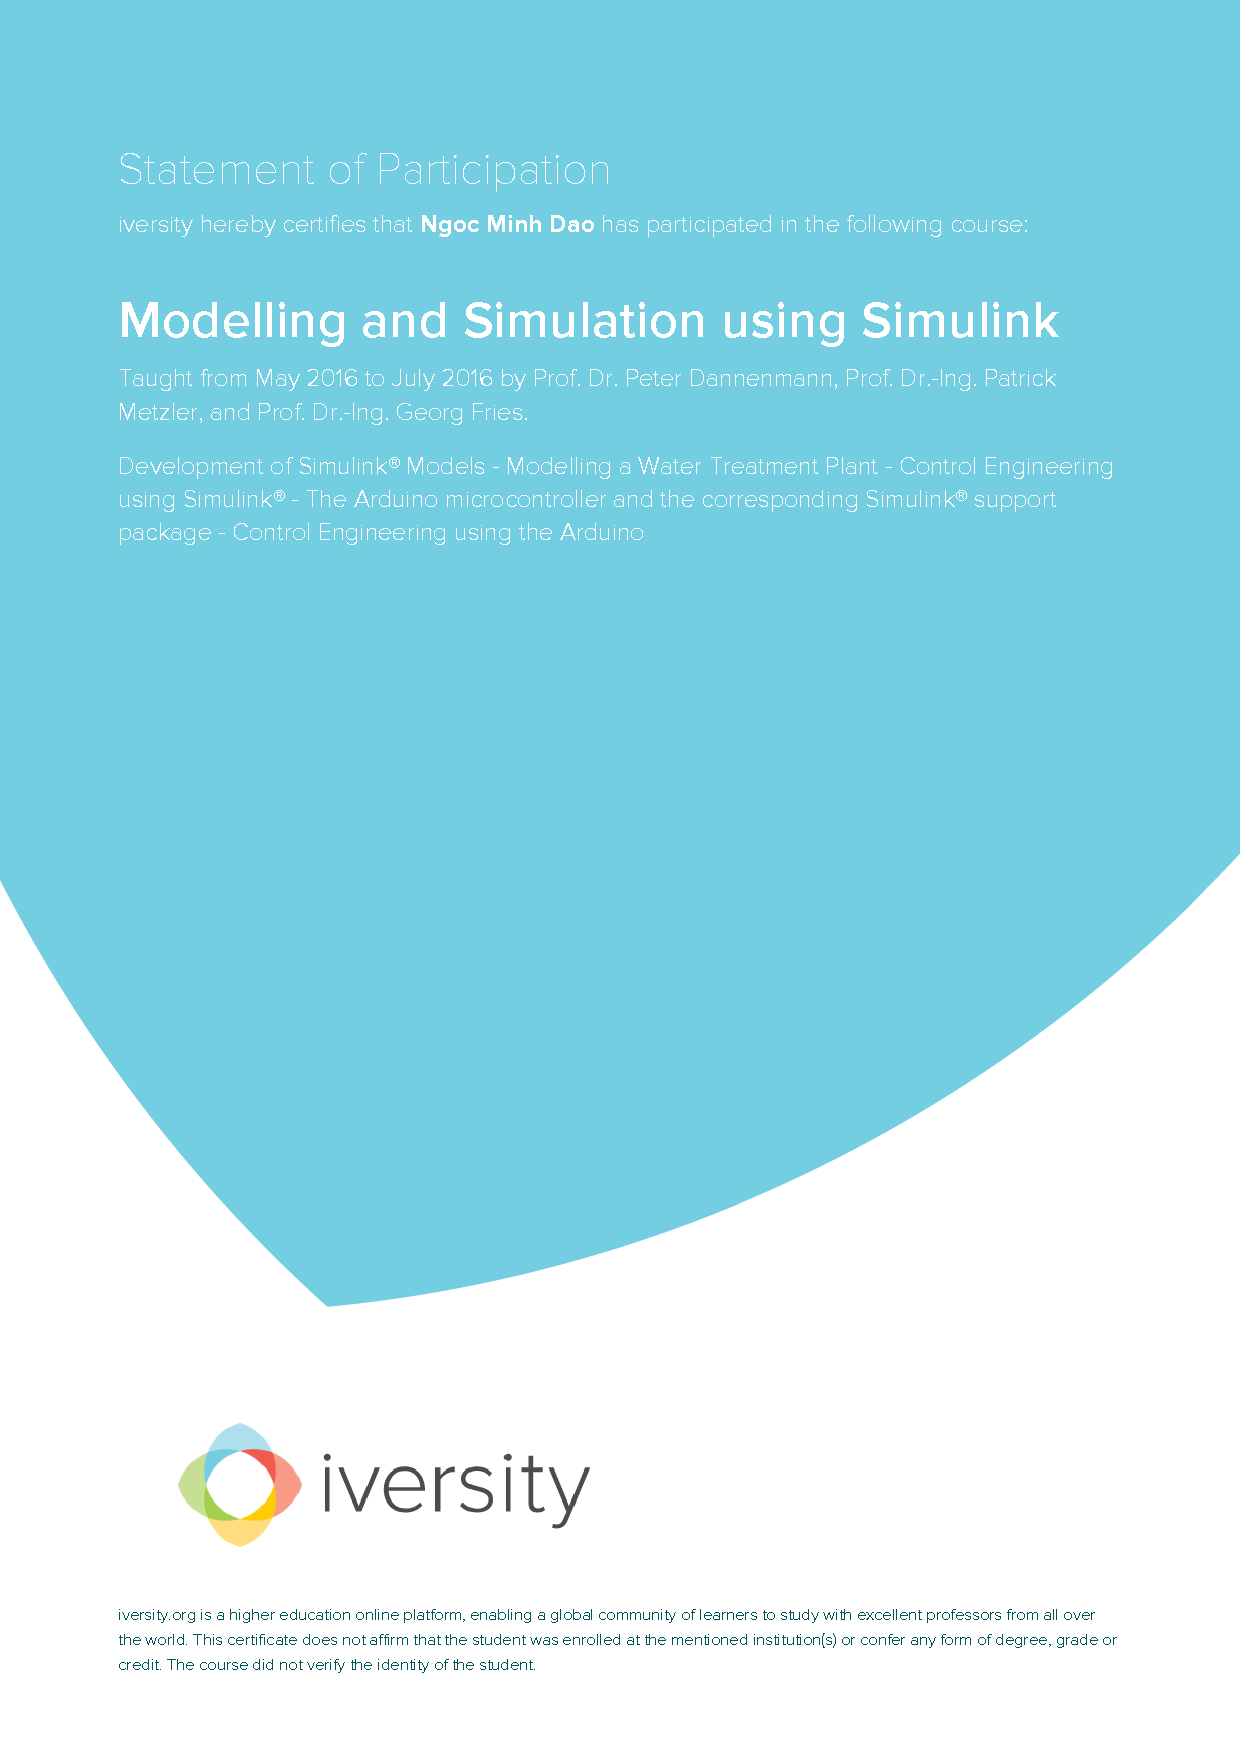
\includepdf [landscape=false, pages=-1] {./zeugnisse/modelling_and_simulation_using_simulink_zertifikat.pdf}
%}}}

% Engagement und Hobbys {{{

% ----------------------------------------
% Schaeffler Automatikgetriebe Schulung
% ----------------------------------------
\newpage
\bookmark[page=\thepage, level=0]{Engagement und Hobbys}
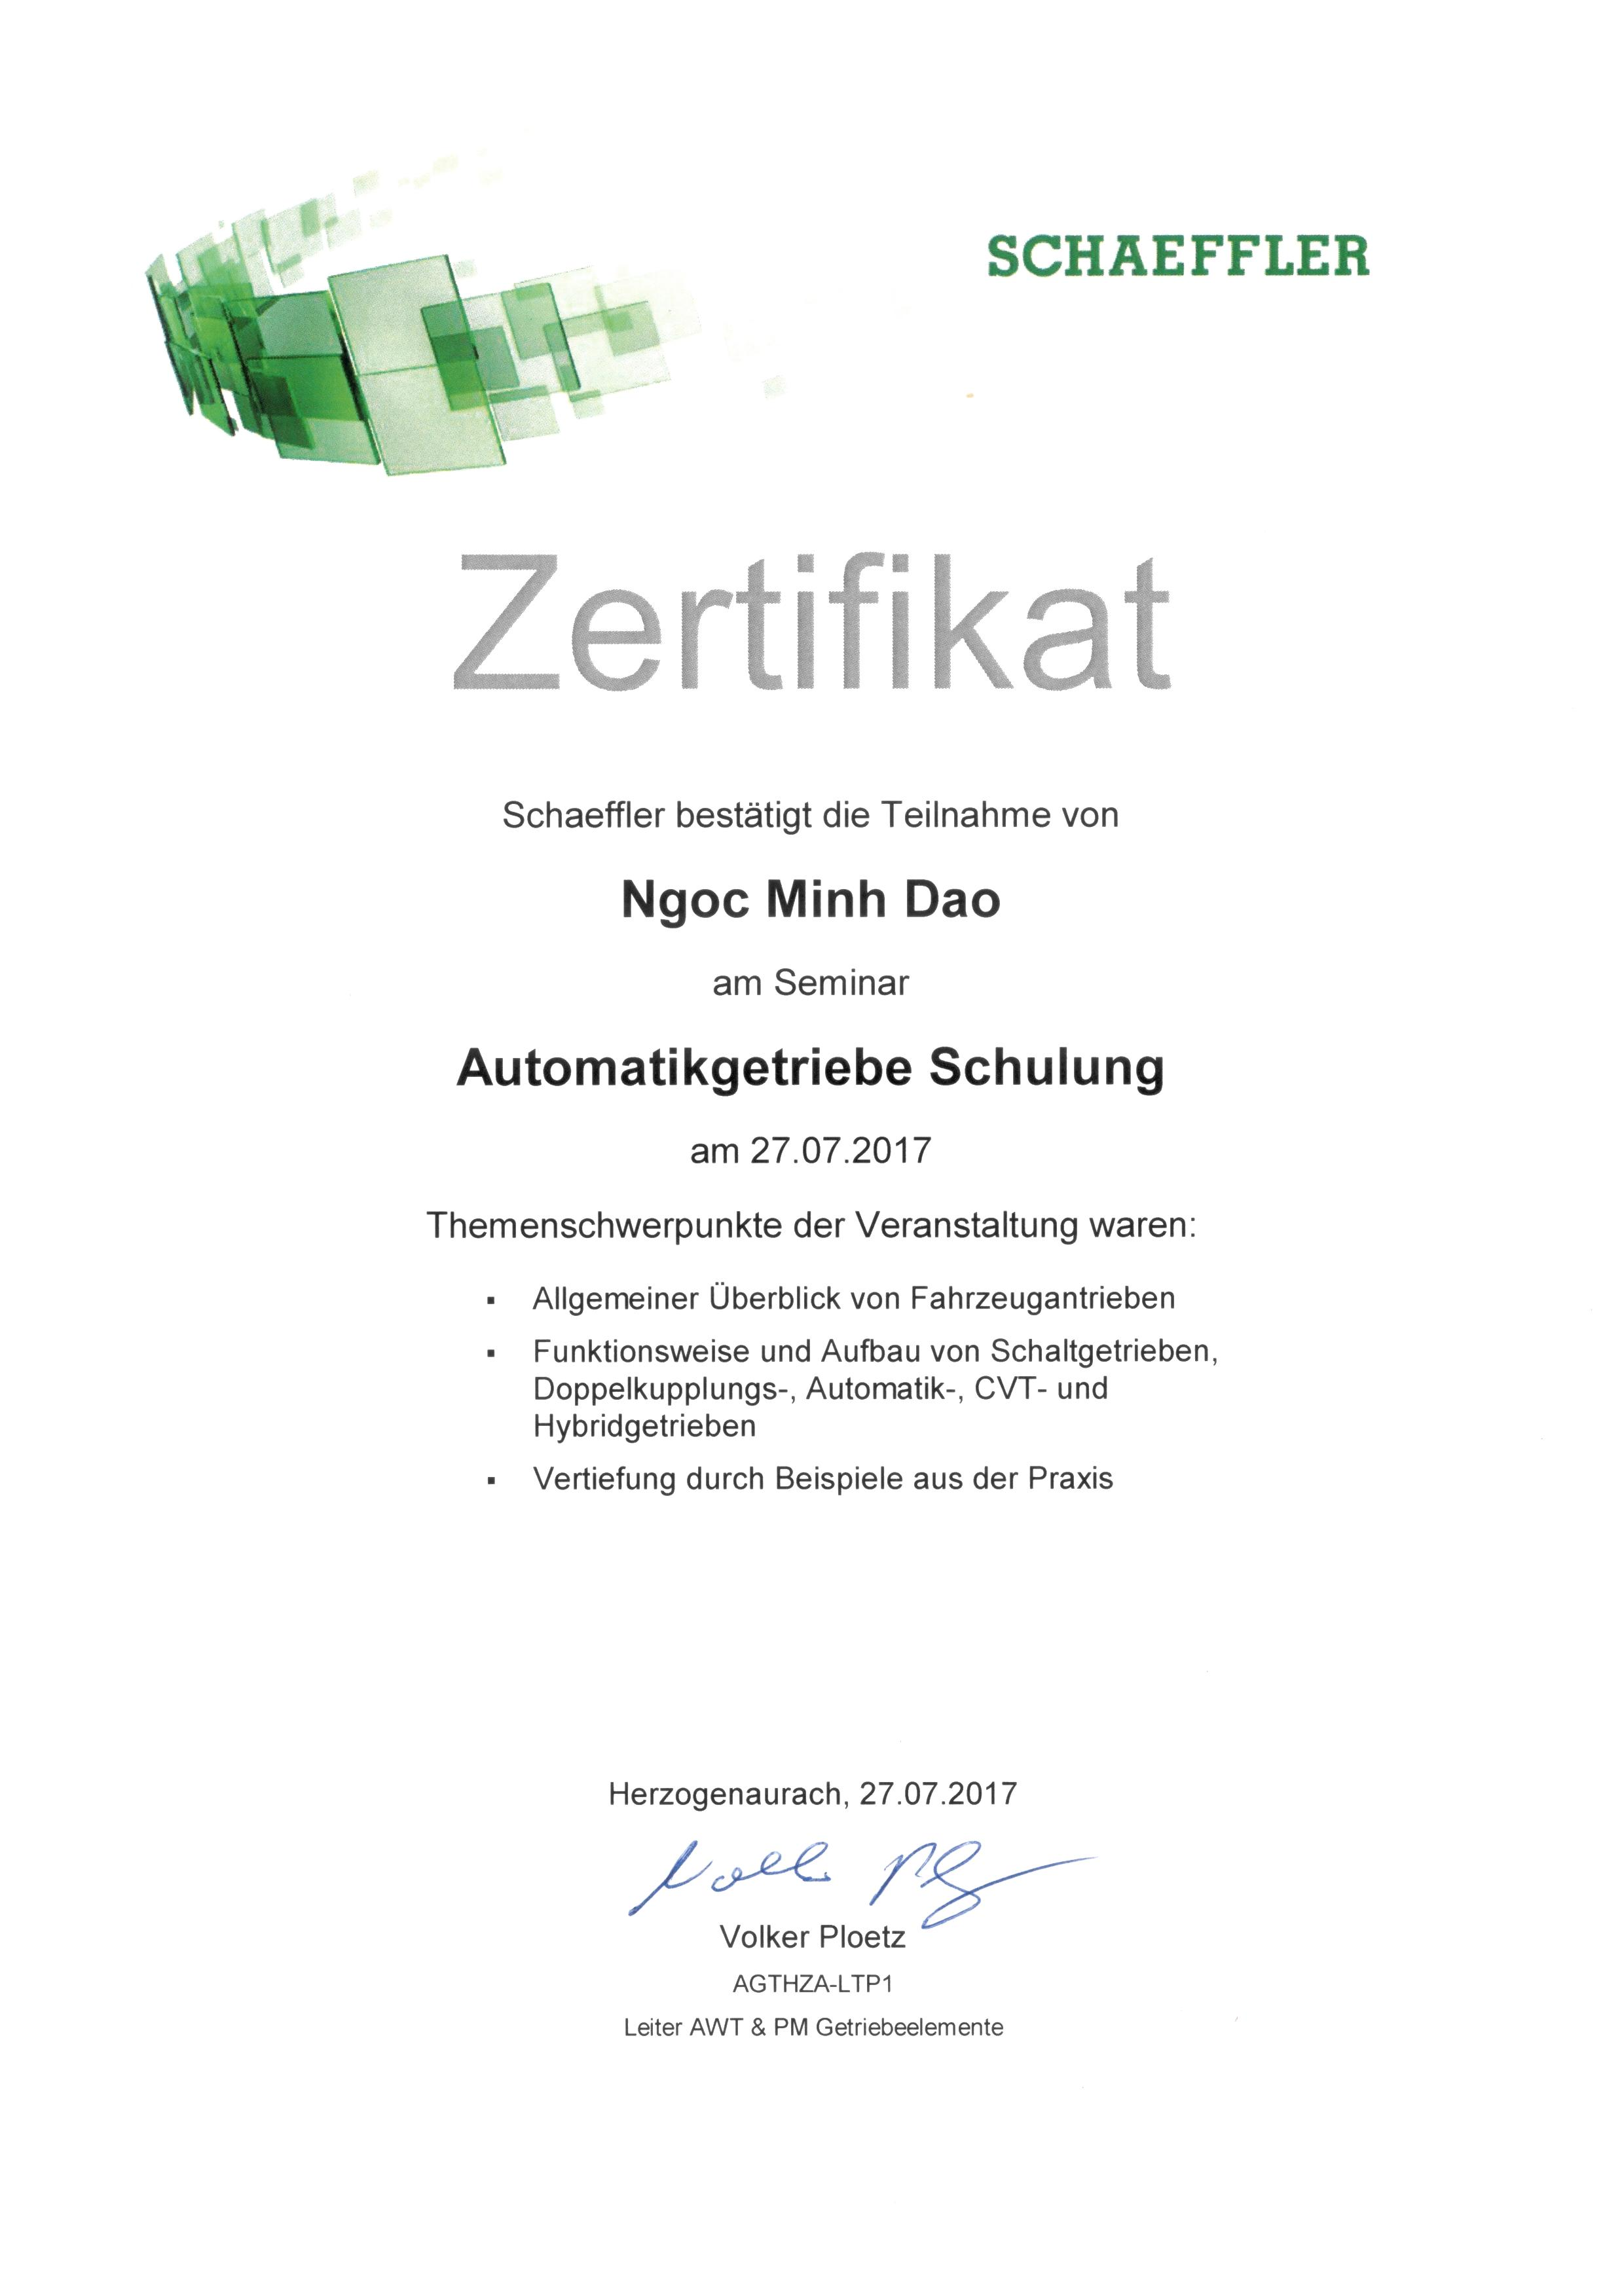
\includegraphics [width=\linewidth, height=\textheight] {./zeugnisse/automatikgetriebe_schulung.jpg}

% ----------------------------------------
% AKAKRAFT Schrauben Kurs
% ----------------------------------------
\newpage
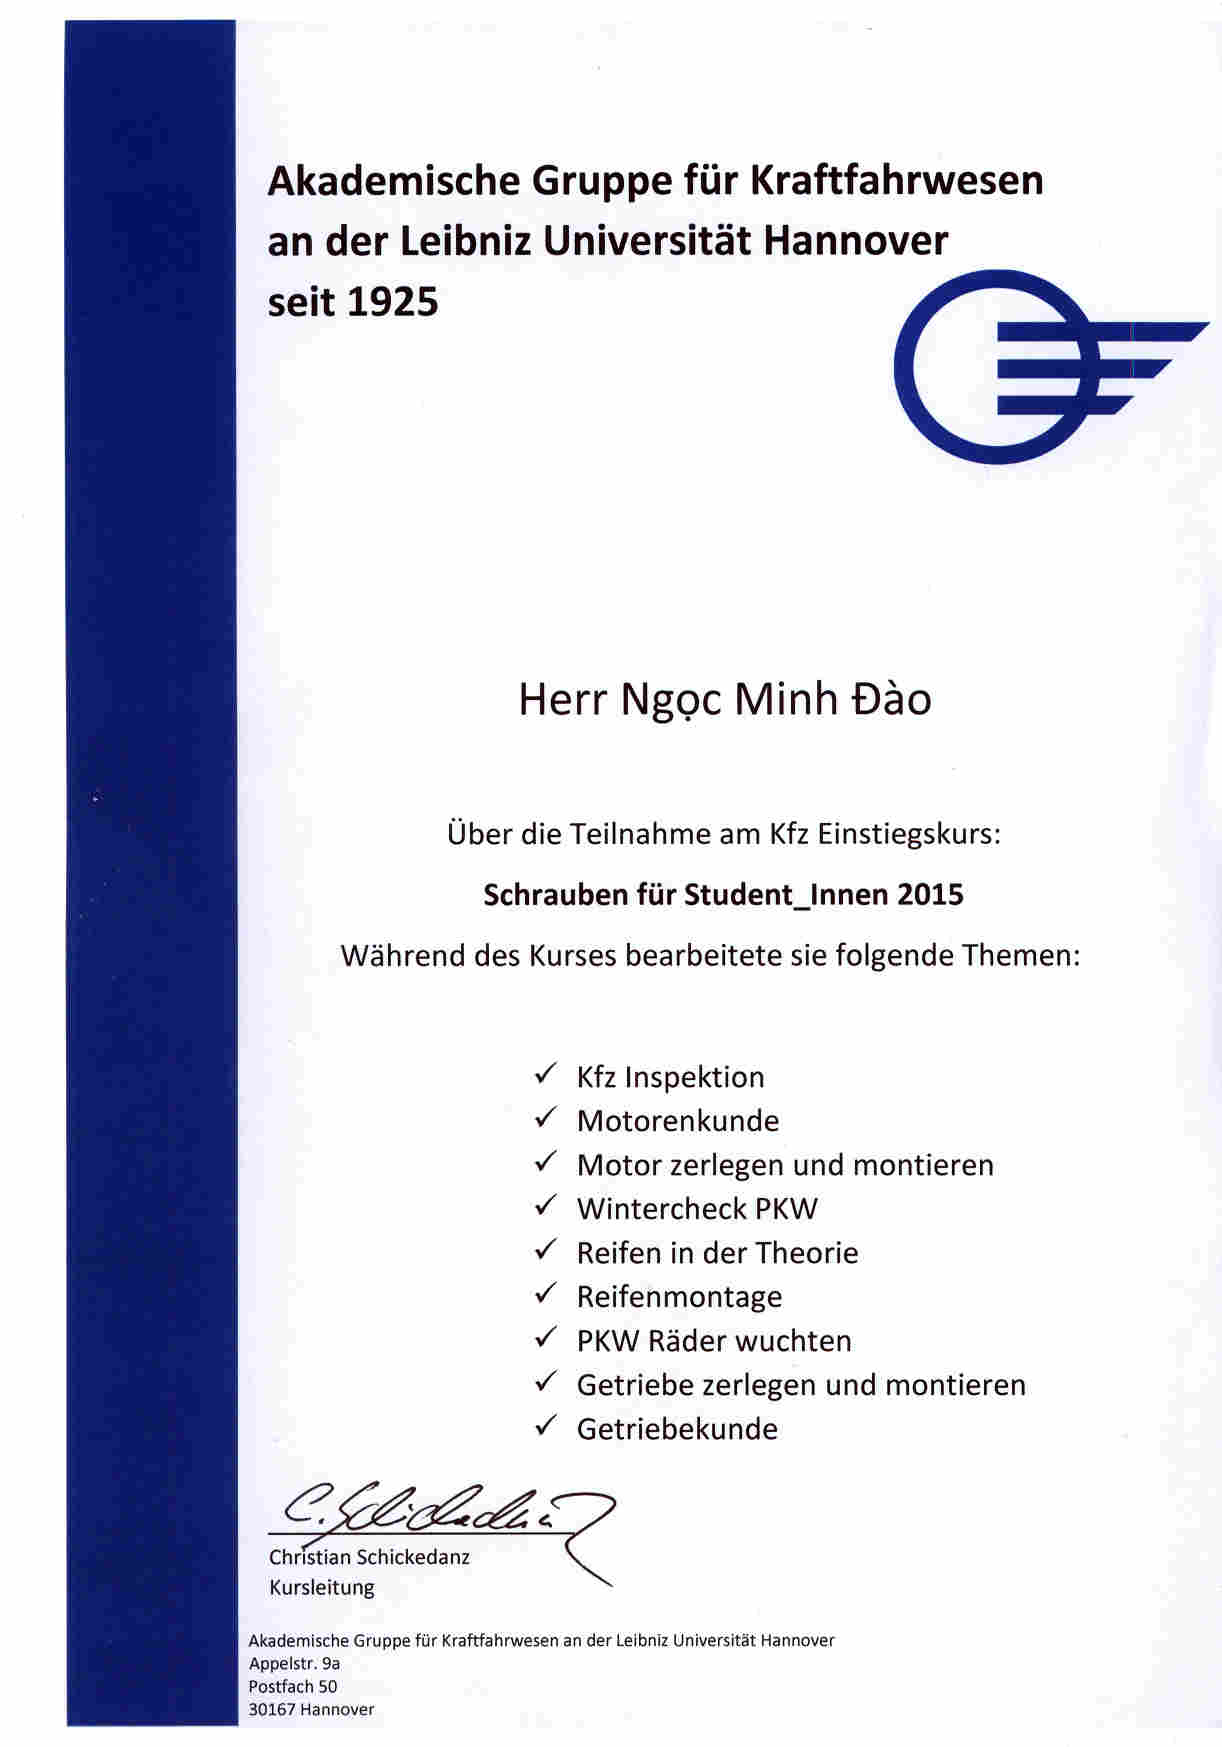
\includegraphics [width=\linewidth, height=\textheight] {./zeugnisse/akakraft_schrauben_kurs_lq.jpg}

% ----------------------------------------
% Schweissenkurs
% ----------------------------------------
\newpage
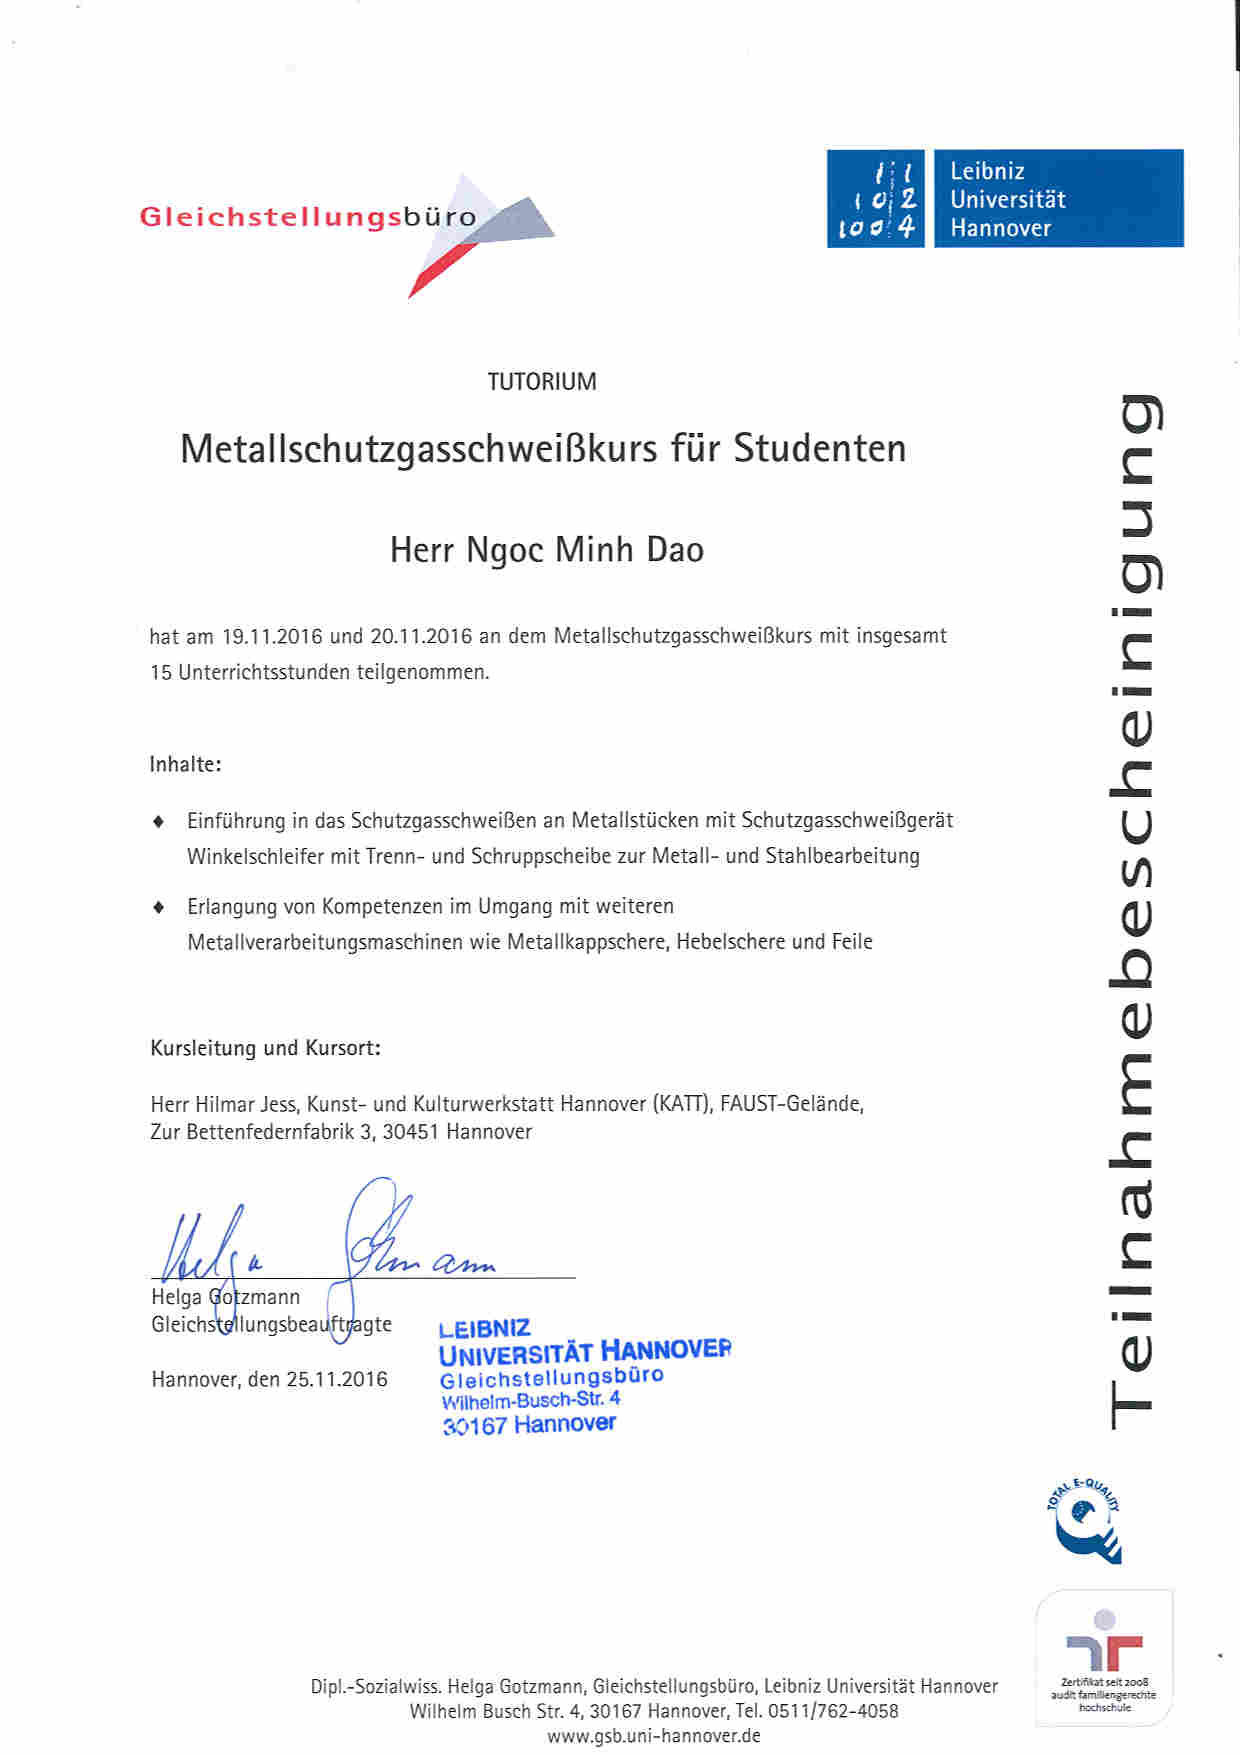
\includegraphics[width=\linewidth, height=\textheight]
{./zeugnisse/schweissenkurs_lq.jpg}

% ----------------------------------------
% Waldfrienden Pokalturnier
% ----------------------------------------
\newpage
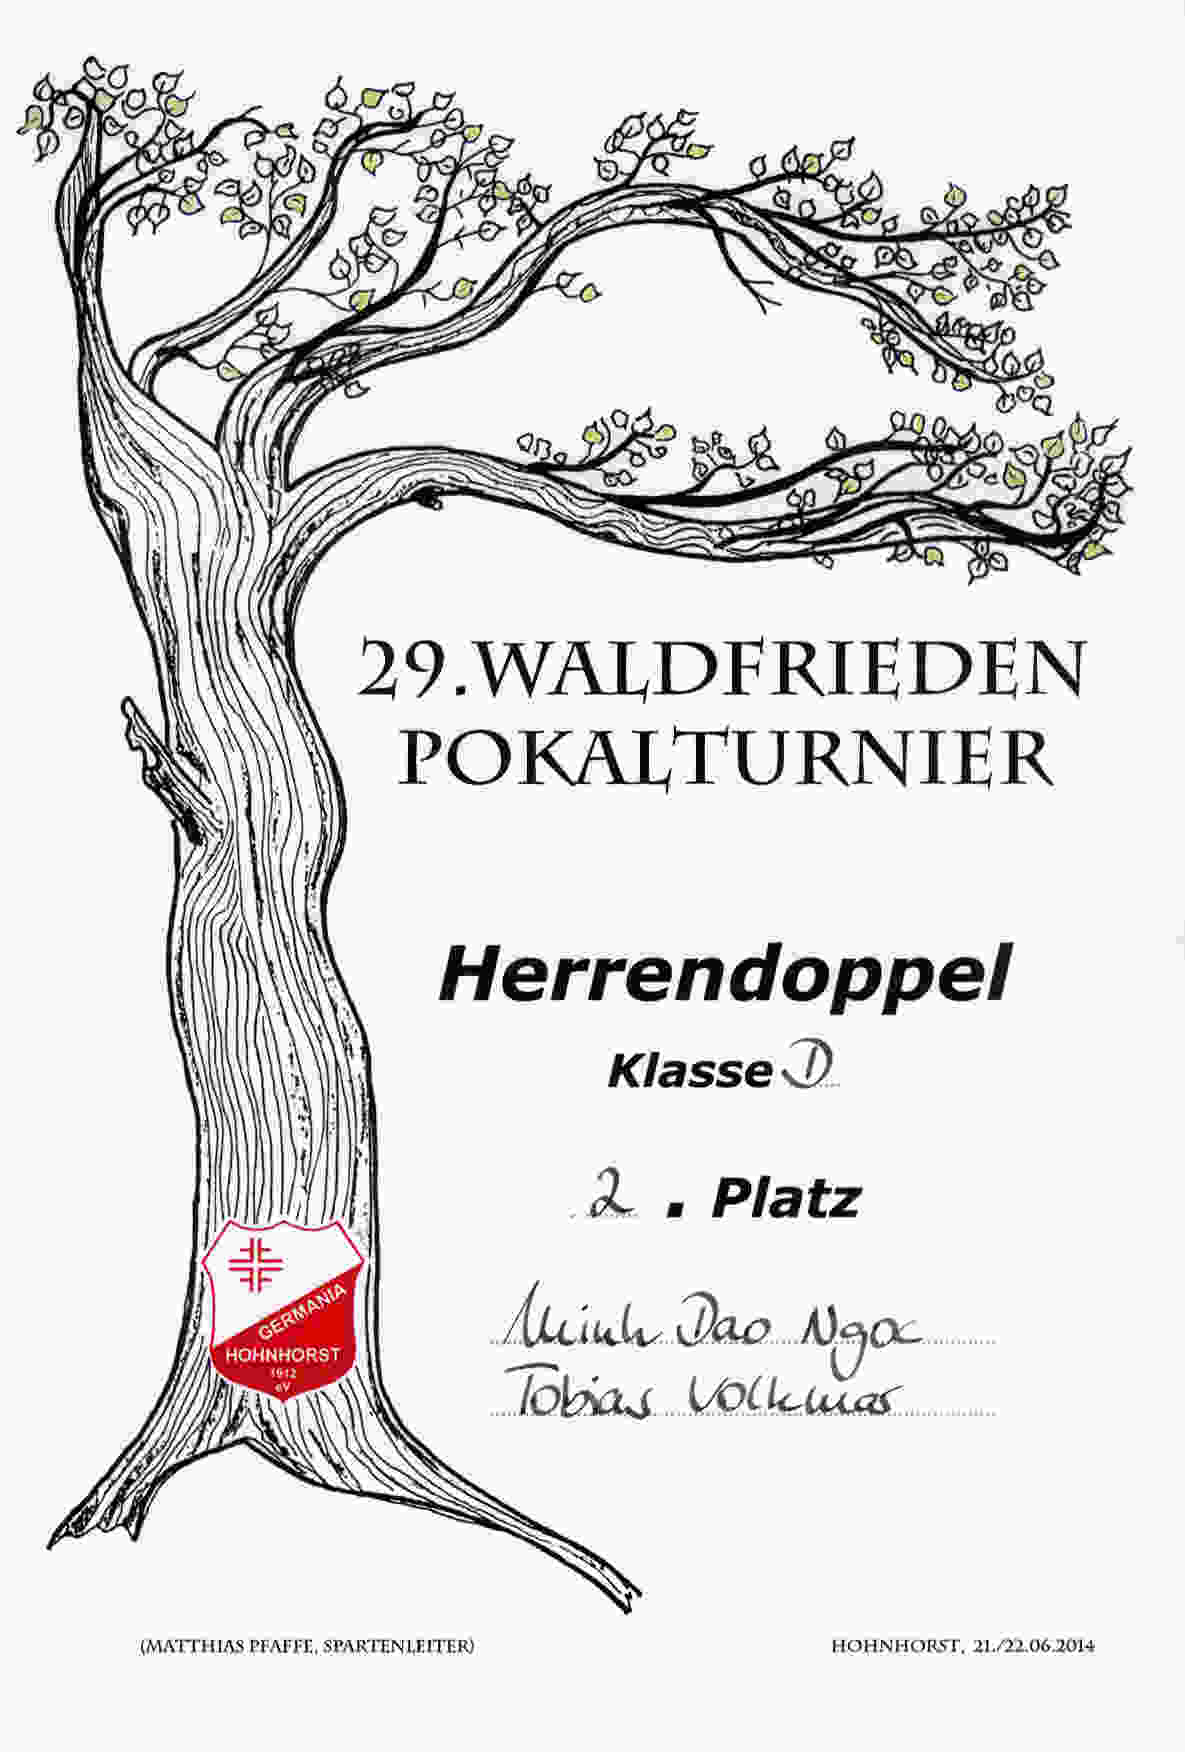
\includegraphics[width=\linewidth, height=\textheight]
{./zeugnisse/29_waldfrieden_pokalturnier_urkunde_lq.jpg}

% }}}

\end{document}
